% Copyright (C) 2014-2023 by Thomas Auzinger <thomas@auzinger.name>

\documentclass[draft,final]{vutinfth} % Remove option 'final' to obtain debug information.

% Load packages to allow in- and output of non-ASCII characters.
\usepackage{lmodern}        % Use an extension of the original Computer Modern font to minimize the use of bitmapped letters.
\usepackage[T1]{fontenc}    % Determines font encoding of the output. Font packages have to be included before this line.
\usepackage[utf8]{inputenc} % Determines encoding of the input. All input files have to use UTF8 encoding.

% Extended LaTeX functionality is enables by including packages with \usepackage{...}.
\usepackage{amsmath}    % Extended typesetting of mathematical expression.
\usepackage{amssymb}    % Provides a multitude of mathematical symbols.
\usepackage{mathtools}  % Further extensions of mathematical typesetting.
\usepackage{microtype}  % Small-scale typographic enhancements.
\usepackage[inline]{enumitem} % User control over the layout of lists (itemize, enumerate, description).
\usepackage{multirow}   % Allows table elements to span several rows.
\usepackage{booktabs}   % Improves the typesetting of tables.
\usepackage{subcaption} % Allows the use of subfigures and enables their referencing.
\usepackage[ruled,linesnumbered,algochapter]{algorithm2e} % Enables the writing of pseudo code.
\usepackage[usenames,dvipsnames,table]{xcolor} % Allows the definition and use of colors. This package has to be included before tikz.
\usepackage{nag}       % Issues warnings when best practices in writing LaTeX documents are violated.
\usepackage{todonotes} % Provides tooltip-like todo notes.
\usepackage{hyperref}  % Enables hyperlinking in the electronic document version. This package has to be included second to last.
\usepackage[acronym,toc]{glossaries} % Enables the generation of glossaries and lists of acronyms. This package has to be included last.
\usepackage{pgfgantt}
\usepackage{xcolor}
\usepackage{listings, listings-rust}
\usepackage{geometry}
\usepackage{eurosym}

% Custom colors for syntax highlighting
\definecolor{codegreen}{rgb}{0,0.6,0}
\definecolor{codegray}{rgb}{0.5,0.5,0.5}
\definecolor{codepurple}{rgb}{0.58,0,0.82}
\definecolor{backcolour}{rgb}{0.95,0.95,0.92}
\definecolor{codered}{rgb}{0.6,0,0}

% Settings for the listings package
\lstdefinestyle{mystyle}{
    backgroundcolor=\color{backcolour},
    commentstyle=\color{codegreen},
    keywordstyle=\color{magenta},
    numberstyle=\tiny\color{codegray},
    stringstyle=\color{codepurple},
    basicstyle=\footnotesize\ttfamily, % Adjust the font size to fit your needs
    breakatwhitespace=false,
    breaklines=true,
    captionpos=b,
    keepspaces=true,
    numbers=left,
    numbersep=5pt,
    showspaces=false,
    showstringspaces=false,
    showtabs=false,
    tabsize=2,
    frame=single,
    language=Rust,
    otherkeywords={self, let, fn, pub, trait, impl, const, mut, constraint}, % Add more keywords as needed
    deletekeywords={data}, % Remove if any conflicts occur
    escapeinside={(*@}{@*)}, % To add LaTeX within your code
    morecomment=[l][\color{codered}]{\#},
}

\lstset{style=mystyle}

% Define convenience functions to use the author name and the thesis title in the PDF document properties.
\newcommand{\authorname}{Àlex Mitjans Llorach} % The author name without titles.
\newcommand{\thesistitle}{Implementation of algebraic cryptographic primitives in the Plonk framework} % The title of the thesis. The English version should be used, if it exists.

% Set PDF document properties
\hypersetup{
    pdfpagelayout   = TwoPageRight,           % How the document is shown in PDF viewers (optional).
    linkbordercolor = {Melon},                % The color of the borders of boxes around hyperlinks (optional).
    pdfauthor       = {\authorname},          % The author's name in the document properties (optional).
    pdftitle        = {\thesistitle},         % The document's title in the document properties (optional).
    pdfsubject      = {Subject},              % The document's subject in the document properties (optional).
    pdfkeywords     = {a, list, of, keywords} % The document's keywords in the document properties (optional).
}

\setpnumwidth{2.5em}        % Avoid overfull hboxes in the table of contents (see memoir manual).
\setsecnumdepth{subsection} % Enumerate subsections.

\nonzeroparskip             % Create space between paragraphs (optional).
\setlength{\parindent}{0pt} % Remove paragraph indentation (optional).

\makeindex      % Use an optional index.
\makeglossaries % Use an optional glossary.
%\glstocfalse   % Remove the glossaries from the table of contents.

% Set persons with 4 arguments:
%  {title before name}{name}{title after name}{gender}
%  where both titles are optional (i.e. can be given as empty brackets {}).
\setauthor{}{\authorname}{}{male}
\setadvisor{Asst. Prof.}{Elena Andreeva}{}{female}

% For bachelor and master theses:
\setfirstassistant{}{Stefano Trevisani}{}{male}
%\setsecondassistant{Pretitle}{Forename Surname}{Posttitle}{male}
%\setthirdassistant{Pretitle}{Forename Surname}{Posttitle}{male}

% For dissertations:
%\setfirstreviewer{Pretitle}{Forename Surname}{Posttitle}{male}
%\setsecondreviewer{Pretitle}{Forename Surname}{Posttitle}{male}

% For dissertations at the PhD School and optionally for dissertations:
%\setsecondadvisor{Pretitle}{Forename Surname}{Posttitle}{male} % Comment to remove.

% Required data.
\setdate{15}{06}{2024} % Set date with 3 arguments: {day}{month}{year}.
\settitle{\thesistitle}{Implementation of algebraic cryptographic primitives in the Plonky2 framework} % Sets English and German version of the title (both can be English or German). If your title contains commas, enclose it with additional curvy brackets (i.e., {{your title}}) or define it as a macro as done with \thesistitle.
%\setsubtitle{}{} % Sets English and German version of the subtitle (both can be English or German).

% Select the thesis type: bachelor / master / doctor.
% Bachelor:
\setthesis{bachelor}
%
% Master:
%\setthesis{master}
%\setmasterdegree{dipl.} % dipl. / rer.nat. / rer.soc.oec. / master
%
% Doctor:
%\setthesis{doctor}
%\setdoctordegree{rer.soc.oec.}% rer.nat. / techn. / rer.soc.oec.

% For bachelor and master:
\setcurriculum{Telecommunications Technologies and Services Engineering}{} % Sets the English and German name of the curriculum.

% Optional reviewer data:
%\setfirstreviewerdata{Affiliation, Country}
%\setsecondreviewerdata{Affiliation, Country}

\begin{document}

\frontmatter % Switches to roman numbering.
% The structure of the thesis has to conform to the guidelines at
%  https://informatics.tuwien.ac.at/study-services

\addtitlepage{english} % English title page.

\begin{abstract*}
As cryptographic technologies evolve, the need for specialized hash functions to operate efficiently over different computational environments become necessary. Traditional symmetric alogrithms like AES and SHA-3 have been optimized for hardware and software implementations, which are designed over binary fields. However, protocols like zero-knowledge proofs require hash functions that are optimised over large prime fields.

This thesis addresses the growing demand for Arithmetization-Oriented (AO) cryptographic hash functions for zero-knowledge applications. The performance and efficiency of many zero-knowledge applications often depends on the efficiency of the hash function used.

In response to this need, this work explores a selection of these hash functions and implements them within two zero-knowledge proving systems: Plonk and Plonky2. The research focuses on benchmarking these hash functions to asses their performance within these sytems. The results obtained provide a fundamental base for future research in the field of zero-knowledge proof technologies, recommending potential areas for further development.

\textbf{Keywords}: Hash functions $\cdot$ Arithmetization-oriented $\cdot$ Plonk $\cdot$ Plonky2 $\cdot$ Zero-knowledge $\cdot$ Arithmetic circuits
\end{abstract*}

\begin{resumen*}
A medida que las tecnologías criptográficas evolucionan, surge la necesidad de funciones hash especializadas para operar eficientemente en diferentes entornos computacionales. Algoritmos simétricos tradicionales como AES y SHA-3 han sido optimizados para implementaciones en hardware y software, enfocándose principalmente en campos binarios. Sin embargo, protocolos como las pruebas de conocimiento cero requieren funciones hash que estén optimizadas sobre grandes campos primos.

Esta tesis aborda la creciente demanda de funciones hash criptográficas orientadas a la aritmetización adaptadas para aplicaciones de conocimiento cero. El rendimiento y la eficiencia de las aplicaciones de conocimiento cero a menudo dependen de la eficiencia de la función hash utilizada.
    
En respuesta a esta necesidad, este trabajo explora una selección de estas funciones hash y las implementa dentro de dos sistemas de prueba de conocimiento cero: Plonk y Plonky2. La investigación se centra en la evaluación comparativa de estas funciones hash para evaluar su rendimiento dentro de estos sistemas. Los resultados obtenidos proporcionan una base fundamental para la investigación futura en el campo de las tecnologías de prueba de conocimiento cero, recomendando áreas potenciales para un desarrollo adicional.

\textbf{Palabras clave}: Funciones hash $\cdot$ Orientado a la aritmetización $\cdot$ Plonk $\cdot$ Plonky2 $\cdot$ Conocimiento cero $\cdot$ Circuitos aritméticos
\end{resumen*}

\begin{resum*}
A mesura que les tecnologies criptogràfiques evolucionen, sorgeix la necessitat de funcions hash especialitzades per operar eficaçment en diferents entorns computacionals. Algorismes simètrics tradicionals com AES i SHA-3 han estat optimitzats per a implementacions en maquinari i programari, centrant-se principalment en camps binaris. No obstant això, protocols com les proves de coneixement zero requereixen funcions hash que estiguin optimitzades sobre grans camps prims.

Aquesta tesi aborda la creixent demanda de funcions hash criptogràfiques orientades a l'aritmetització adaptades per a aplicacions de coneixement zero. El rendiment i l'eficiència de les aplicacions de coneixement zero sovint depenen de l'eficiència de la funció hash utilitzada.
    
En resposta a aquesta necessitat, aquest treball explora una selecció d'aquestes funcions hash i les implementa dins de dos sistemes de prova de coneixement zero: Plonk i Plonky2. La investigació es centra en l'avaluació comparativa d'aquestes funcions hash per avaluar el seu rendiment dins d'aquests sistemes. Els resultats obtinguts proporcionen una base fonamental per a la recerca futura en el camp de les tecnologies de prova de coneixement zero, recomanant àrees potencials per a un desenvolupament addicional.

\textbf{Paraules clau}: Funcions hash $\cdot$ Orientat a l'aritmetització $\cdot$ Plonk $\cdot$ Plonky2 $\cdot$ Coneixement zero $\cdot$ Circuits aritmètics
\end{resum*}

\begin{acknowledgements*}
First of all, I wish to express my appreciation to my advisor, Prof. Elena Andreeva, for providing me with her guidance and the opportunity to conduct my thesis within her research group. I would also like to thank Stefano Trevisani for his advice and for assisting me with technical issues that arose during my thesis.

Finally, I would like to thank my family for their support and belief in me throughout my studies, and for making this incredible experience in Vienna possible.
\end{acknowledgements*}

% Select the language of the thesis, e.g., english or naustrian.
\selectlanguage{english}

% Add a table of contents (toc).
\setcounter{tocdepth}{2}
\tableofcontents % Starred version, i.e., \tableofcontents*, removes the self-entry.

% Switch to arabic numbering and start the enumeration of chapters in the table of content.
\mainmatter

\chapter{Introduction}
\section{Motivation}
The interest in zero-knowledge proofs has experienced a notable growth, especially with the increasing interest in blockchain technology and verifiable computation. Although this technology was first described by Goldwasser et al. in 1985, blockchain technology has helped zero-knowledge proofs increase his popularity. Today, this technology is widely used across various industries, from Web3 platforms to supply chains and the Internet of Things (IoT).

In the world of blockchain technology, zero-knowledge proofs play a crucial role in enhancing privacy and security. They enable participants to prove the validity of transactions or computations without revealing sensitive or private information, therefore addressing concerns regarding data privacy and confidentiality.

Moreover, in IoT networks, they can prove and verify the authenticity of exchanged data. Similarly, in supply chains, zero-knowledge proofs are used to validate product authenticity while mantaining privacity.

Cryptographic hash functions play a fundamental role in ensuring the integrity and security of digital data. These functions are widely employed in various cryptographic protocols, digital signatures, messages and passwords verification, for example.
Hash functions such as SHA-2 or SHA-3, while widely used and secure, may not meet the efficient requirements of zero-knowledge proofs. This has led to the development of zero-knowledge friendly hash functions such as Poseidon, Arion and Griffin to name a few, which offer compact arithmetic circuits, enabling faster proof generation and verification within zero-knowledge proof systems. 

\section{Statement of purpose}
This thesis aims to investigate some of the most used and novel hash functions efficient in zero-knowledge and implement them within a zero-knowledge framework. Specifically, the obejctives of this research include the plain implementation of these hash functions in the Goldilocks field and the BLS12-381 scalar field. Subsequently, these hash functions will also be implemented in two zero-knowledge frameworks, Plonk and Plonky2.\\
Furthermore, benchmarks have been done to asses the performance of these hash functions in plain performance and within these frameworks.

\section{Outline}
This thesis is organized as follows. We begin by presenting the necessary background knowledge and defining all the concepts used throughout this thesis in Chapter~\ref{sec:theory}. Then, in Chapter~\ref{sec:proof-theory}, we explain proofs systems, define zero-knowledge proofs, SNARKs, and specifically, the proof system that we will use, Plonk. In Chapter~\ref{sec:zk-hashes}, we define the hash functions that will be implemented in this thesis and provide all the necessary theoretical knowledge to understand them. Next, in Chapter~\ref{sec:impl}, we explain how we developed these hash functions, including some of the parameters used for their implementation. In Chapter~\ref{sec:evaluation}, we present and discuss the results obtained from the benchmarks. Next, conclusions are developed togheter with some insights for future work in Chapter~\ref{sec:conclusions}. Finally, in Chapter~\ref{sec:sustainability}, we detail a sustainability analysis and ethical implications of ower project.

\section{Work plan}
The work on this thesis has been organized according to the schedule in Figure~\ref{fig:gant}.

    \begin{figure}[htbp]
        \begin{center}
            \makebox[\textwidth]{\begin{ganttchart}[
                y unit title=0.4cm,
                y unit chart=0.5cm,
                vgrid,hgrid,
                title label anchor/.style={below=-1.6ex},
                title left shift=.05,
                title right shift=-.05,
                title height=1,
                progress label text={},
                bar height=0.7,
                group right shift=0,
                group top shift=.6,
                group height=.3
                ]{1}{23}
                %labels
                \gantttitle{Thesis Phases} {23} \\
                \gantttitle{2024} {23} \\
                \gantttitle{February}{5} 
                \gantttitle{March}{5}
                \gantttitle{April}{5}
                \gantttitle{May}{5}
                \gantttitle{June}{3} \\
                %tasks
                %First group
                \ganttgroup{Research}{1}{6} \\
                \ganttbar{Literature review}{1}{6} \\\\

                %Second group
                \ganttgroup{Plonky2 Implementation}{3}{13} \\
                \ganttbar{Hades}{5}{6} \\
                \ganttbar{Poseidon}{5}{8} \\
                \ganttbar{Rescue}{8}{9} \\
                \ganttbar{Griffin}{9}{9} \\
                \ganttbar{Anemoi}{9}{11} \\
                \ganttbar{Arion}{11}{13} \\\\

                \ganttgroup{Plonk Implementation}{13}{16} \\
                \ganttbar{Hash functions}{13}{16} \\\\

                %Third group
                \ganttgroup{Performance}{11}{14} \\
                \ganttbar{Optimizations}{11}{14} \\\\

                %Fourth group
                \ganttgroup{Benchmarking}{13}{17} \\
                \ganttbar{Tests}{13}{17} \\\\

                %Fourth group
                \ganttgroup{Documentation}{19}{22} \\
                \ganttbar{Thesis}{19}{22} \\
            
            \end{ganttchart}}
        \end{center}
        \caption{Gantt Chart}
        \label{fig:gant}
    \end{figure}

\chapter{Preliminaries}
\label{sec:theory}
In this chapter, we provide some background knowledge that will be required for understanding future parts of the thesis.

\section{Hash Functions}
A bit-oriented hash function~\cite{preneel1994cryptographic} is a mathematical function $H : \{0,1\}^* \rightarrow \{0,1\}^n$ with $n\geq1$ which takes an input (or 'message') of variable length and computes a fixed length output.

A hash function generally starts by dividing the input data into fixed size blocks. This is necessary because hash functions operate on data with a fixed length, and the input could be of any length. This padding process varies depending on the details of the hash function.

\subsection*{Properties}
To be an effective cryptographic tool, the hash function needs to posses the following properties~\cite{preneel1993analysis}:
\begin{itemize}
    \item \textbf{One way function (pre-image resistance):} It should be computationally difficult to reverse a hash funtion.
    \item \textbf{Target collision resistance (Second pre-image resistance):} Given an input and its hash, it should be computationally difficult to find a different input with the same hash.
    \item \textbf{Collision resistance:} It should be computationally difficult to find two different inputs of any arbitrary length that result in the same hash value.
    \item \textbf{Deterministic:} The same input will always produce the same output.
    \item \textbf{Efficiency:} The hash function must compute values quickly to ensure practical usability.
\end{itemize}

\subsection{Block ciphers}
Block ciphers~\cite{knudsen1999block} are symmetric key cryptographic alogrithms that operates on fixed length groups of bits, called blocks. The alogrithm accepts an input block of size $n$ bits and a key of size $k$ bits, and produce an $n$ bits output block. They are designed to be reversible, meaning the ciphertext can be transformed back into the plaintext using the same key.
\begin{equation}
    E:\{0,1\}^k\times\{0,1\}^n\rightarrow\{0,1\}^n.
\end{equation}

Block ciphers usually use multiple rounds of operations, including permutations and substitutions, until inverting the function becomes hard. They can be used to construct hash functions.

\textit{Feistel networks}, \textit{Substitution-Permutation Networks} (SPNs), \textit{Horst} schemes and \textit{open Flyestel} components are fundamental structures used to design block ciphers.

\subsubsection*{Feistel Networks}
A Feistel network~\cite{10.1007/BFb0034838, feistel1973cryptography} is a structure used to construct block ciphers. The input block $X$ is divided into two parts $X_1\text{ and }X_2$. One round of a Feistel network is defined as follows:
\begin{flalign*}
    Y_1=X_1\oplus F(X_2,K) \\
    Y_2=X_2 \\
    Y_1'=Y_2 \\
    Y_2'=Y_1,
\end{flalign*}
where $K$ is the round key, $F$ is the round function and $(Y_1',Y_2')$ is the data output of the round taken as input to the next round.

The Feistel network provides difussion of the input blocks. After two rounds of the network the dissufion is complete, that is, both output blocks depend on both input blocks.

\subsubsection*{Substitution-permutation network}
Substitution-permutation network (SPN)~\cite{feistel1973cryptography, shannon1949communication} is used to generate block ciphers. It is a repeated series of mathematical operations.

SPN takes an input block of the plaintext and a key as the input, and applies substitution (S-box) and Permutation (P-box) to each round.\\
An \textbf{S-box} substitues each byte of the input block with another byte. This layer of the SPN introduces non-linearity.\\
A \textbf{P-box} is a permutation of every bit: the bits of the S-box output are permuted, and then are passed to the S-box of the next round.

Thus, in SPN consists on three primary operations in each round: addition of a round key, substitution and permutation.

\subsubsection*{Horst scheme}
\label{sec:horst}
Horst is another structure that can be used to design block ciphers, it is defined in~\cite{grassi2022horst} and used in the Griffin hash function design. Let $t\geq2$. For each $i\in{1,2,\dots,t-1}$, let $G_i:\mathbb{F}_q^i\rightarrow\mathbb{F}_q\backslash\{0\}$ and $\mathbb{F}_i:\mathbb{F}_q^i\rightarrow\mathbb{F}_q$. Horst is defined over $\mathbb{F}_q^t$ as $x=(x_0,\dots,x_{t-1})\mapsto y=(y_0,\dots,y_{t-1})$, where
\begin{equation*}
    y_i:=\begin{cases}
        x_{i+1}\cdot G_{i+1}(x_0,x_1,\dots,x_i)+F_{i+1}(x_0,x_1,\dots,x_i) & \text{if } i\in{0,1,\dots,t-2}, \\
        x_0 & \text{otherwise } (i=t-1).
    \end{cases}
\end{equation*}

The final circular shift is crucial for achieving full diffusion (as in the case of any Feistel scheme), but it can be replaced with a different linear diffusion.

\subsubsection*{Open Flyestel structure}
\label{sec:flyestel}
The \textit{open Flyestel} structure is a non-linear component presented and used in the design of Anemoi~\cite{bouvier2023new}.

Let $Q_\gamma:\mathbb{F}q\rightarrow\mathbb{F}_q$ and $Q_\delta:\mathbb{F}_q\rightarrow\mathbb{F}_q$ be two quadratic functions, and let $E:\mathbb{F}_q\rightarrow\mathbb{F}_q$ be a permutation. Then, the \textit{Flyestel} is a pair of functions relying on $Q_\gamma, Q_\delta$ and $E$. The \textit{open Flyestel} is the permutation of $(\mathbb{F}_q)^2$ obtained using a 3-round Feistel network with $Q_\gamma, E^{-1}$, and $Q_\delta$ as round functions. It is defined as $\mathcal{H}(x,y)=(u,v)$.
\begin{equation}
    \begin{cases}
        x\leftarrow x-Q_\gamma(y), \\
        y\leftarrow y-E^{-1}(x), \\
        x\leftarrow x+Q_\delta(y), \\
        u\leftarrow x,v\leftarrow y.
    \end{cases}
\end{equation}

\section{Sponge structure}
\label{sec:sponge-construction}
The sponge construction will be used in the different hash functions that are implemented on this thesis.

\subsection*{Overview}
The sponge construction maps an input of arbitrary length to an arbitrary length output. So the input don't have any restriction of his length, and the output length is not determined by the input~\cite{guido2011cryptographic}.

The sponge construction is built over an internal permutation, $\mathcal{P}$, that operates on the $\mathbb{F}_q^{r+c}$. This permutation works on a state with a length of $t$ called the width, where $t=r+c$, $r$ is the rate (outer part of the state) and $c$ the capacity (inner part of the state). The digest consists of $h$ elements.

A sponge can be used to obtain hash function: you use the sponge to absorb the input data, and then squeeze out just enough to form a hash. This approach enables hash functions to handle inputs of varying lengths while producing fixed-length outputs.
Figure~\ref{fig:sponge-hash} explains the principle of the Sponge construction.

First, the state is initialized to zero, and the following operations are made to the input message $m$:
\begin{enumerate}
    \item \textbf{Padding:} The padding rule of the sponge works as follows: when the length of the input message is not a multiple of the rate of the sponge, we append 1$\in\mathbb{F}_q$ to the input followed by enough zeros to make it a multiple of $r$, and split the message into blocks of size $r$, called chunks.
    \item \textbf{Absorbing:} When the input is divided into blocks of size $r$ (chunks), they are absorbed into the state of the sponge construction. Each one of these blocks is added to the outer part of the state using vector addition in $\mathbb{F}^r$ (where $\mathbb{F}$ is a finite field), and then the permutation is applied to it. This process is repeated for each block.
    \item \textbf{Squeezing:} In this phase the output is produced by extracting min$\left(h,r\right)$ elements from the outer part of the state $r$. If $r<h$, we apply the permutation $\mathcal{P}$ and extract the $r$ elements, this process is repeated until we reach the desired output length $h$.
\end{enumerate}
The length of the output, $h$, can be arbitrarily chosen.

\begin{figure}[htbp]
    \centering
    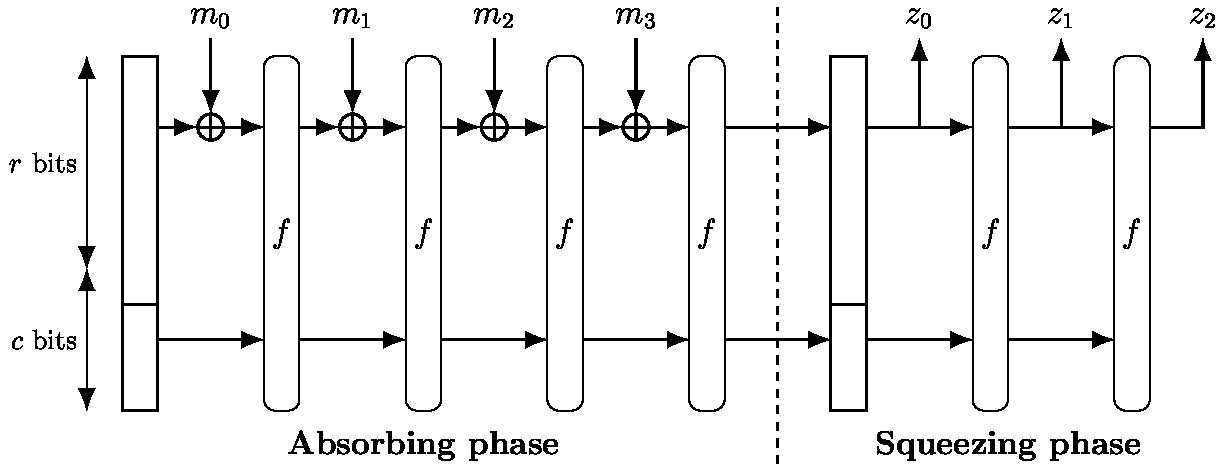
\includegraphics[width=\textwidth]{graphics/sponge.png}
    \caption{Sponge construction with 4 input chunks and a permutation $f$.}
    \label{fig:sponge-hash}
\end{figure}

\subsection{Cryptographic permutation}
A cryptographic permutation is a function that maps an input to an unique output of the same length. The function is designed to be bijective, every input has a unique output. It consists in a sequence of operations iterated over $R$ rounds. This sequence of operations are called the round function.

Some of the most typical elements that will be used in the implemented hash functions are:

\subsubsection*{Non-linear layer (S-box)}
\label{sec:s-box}
In the designs of S-boxes, functions like $f(x)=x^\alpha$ over finit fields $\mathbb{F}_p$ are often used. These functions must be bijective, to be suitable for cryptographic purposes. To ensure that it is bijective, \textit{Fermat's Little Theorem}~\cite{daepp2011fermat} is used along with specific properties of finite fields.

\textit{Fermat's Little Theorem} states that if $p$ is a prime number and $a$ is an integer such that $a$ is not divisible by $p$, then:
\begin{equation}
    a^{p-1}\equiv1\text{ }(\text{mod }p)
\end{equation}

The condition gcd$(\alpha,p-1)=1$ ensures that the funciton $f(x)=x^\alpha$ is a permutation of the field $\mathbb{F}_p$. Next, a detailed explanation is provided:
\begin{itemize}
    \item The condition gcd$(\alpha,p-1)=1$ guarantees that $\alpha$ has a multiplicative inverse modulo $p-1$. This means there exists an integer $\beta$ such that:
    \begin{equation}
        \alpha\cdot\beta\equiv1\text{ }(\text{mod }p-1).
    \end{equation}
    This inverse $\beta$ allows us to define the inverse function $g(x)=x^\beta$. Consequently, $f(g(x))=g(f(x))=x$, proving that $f(x)=x^\alpha$ is bijective.
    \item For $f(x)=x^\alpha$ to be a permutation, the mapping $x\mapsto x^\alpha$ must cover all elements of $\mathbb{F}_p$. Thus, if gcd$(\alpha,p-1)\neq1$, there would exists some $a,b\in\mathbb{F}_p$, such that $a^\alpha=b^\beta$ for $a\neq b$, not satisfying the property. 
\end{itemize}

\subsubsection*{Constant addition}
This component of the permutation consists on the addition of a constant to the state of the sponge, how to add this constant and when depends on the design of the hash function.
\begin{equation}
    \text{state}=\text{state}\oplus c_i
\end{equation}
The round constants, $c_0,\dots,c_{R-1}$, are fixed and public.

\subsubsection*{Liner Layer}
The linear layer consists on the computation of a matrix times vector multiplication.\\ The matrix depends on the design of the hash function, although it is usually a \textit{Maximum Distance Separable} (MDS) matrix~\cite{duval2018mds} and the vector is the state of the sponge.

A \textit{Maximum Distance Separable} matrix is a type of matrix that provides diffusion properties. It has the property that every square submatrix is invertible. This means that each output bit depends on all input bits. Thus, it ensures that small changes in input lead to significant changes in the output.

\section{Finite fields}
\label{sec:finite-fields}
This section aims to provide and overview of finite fields and offer a brief introduction to the Goldilocks field and the BLS12-381 elliptic curve. As the focus of this thesis does not include elliptic curves and their associated mathematics, we limit it to essentials concepts. The definitions provided in this section will be used through the rest of the document.

\subsection*{Overview}
A field $\mathbb{F}$ in mathematics is a set on which operations such as addition, multiplication, division and substraction are defined.

A finite field $\mathbb{F}_q$ is a field that contains a finite number of elements, $|\mathbb{F}_q| \in\mathbb{N}$. The number of elements in the field is also called \textit{order}, and for a finite field of \textit{order} $q$, it exists if $q=p^k$, where $p$ is a prime number and $k\in\mathbb{N}$~\cite{cramer1998zero}.

Next we will focus on two types of finite fields:
\begin{itemize}
    \item \textbf{Prime Fields}. They are constructed over a prime number of elements. The finite field $\mathbb{F}_p$, denotes the prime field, where $p$ is a prime number. The elements of $\mathbb{F}_p$ range from $0$ to $p-1$.\\
    There is an important property of prime field that makes them suitable for cryptography: anytime you perform a mathematical operation such as addition, multiplication, division or substraction with another element from the same prime field, it will lead to an element that also belongs to the prime field.
    \item \textbf{Binary Fields}. The elements of this field are binary polynomials with coeficients being 0 or 1. It is defined as $\mathbb{F}_{2^n}$, where $n$ is an arbitrary integer and it constains 2$^n$ elements, represented as $n$-bits string, where the degree of each polynomial is at most $n-1$.\\
    In modulo 2 arithmetics, $1+1\equiv\text{0 mod2}, 1+0\equiv\text{1 mod2}, 0+0\equiv\text{0 mod2}$, so addition in $\mathbb{F}_{2^n}$ is a XOR operation.
\end{itemize}

\subsection{Goldilocks field}
\label{sec:goldilocks}
The Goldilocks field is a prime field denoted as $\mathbb{F}_p$, where $p=2^{64} - 2^{32} + 1$. Due to its specific form, this field allows for efficient arithmetic operations.

\subsection{BLS12-381}
\label{sec:bls12}
BLS12-381~\cite{cryptoeprint:2017/1050} is a pairing-friendly elliptic curve.
The field modulus $q$ is a prime and has 383 bits or fewer, and the subgroup size $p$ is also a prime and has 256 bits or fewer.
\[
\begin{split}
    q=\mathtt{0x1a0111ea397fe69a4b1ba7b6434bacd764774b84f38512bf} \\
    \mathtt{6730d2a0f6b0f6241eabfffeb153ffffb9feffffffffaaab}
\end{split}
\]
\[
\begin{split}
    p=\mathtt{0x73eda753299d7d483339d80809a1d80553bda402f}
    \\
    \mathtt{ffe5bfeffffffff00000001}
\end{split}
\]

\chapter{Proof Systems}
\label{sec:proof-theory}
\section{Zero Knowledge Proofs}
\subsection*{Overview}
This concept was introduced by Goldwasser et al.~\cite{goldwasser1985knowledge} in 1985, which provided a widely used definition of zero-knowledge protocols: "A zero-knowledge proof allows one party (the prover) to convince another party (the verifier) of the truth of a statement without disclosing any information other than the fact that the statement is indeed true".\\To ensure this the prover constructs a new statement, known as a proof of knowledge, whose truth implies the truth of the original statement, without divulging any private information.

First we will explain Interactive proofs systems, required for explaining SNARKs, and their role in zero-knowledge proofs.

\subsection{Interactive Proof System}
An interactive proof system models an interaction between two parties: the prover and the verifier. The prover wants to convince the verifier of the truth of a statement, and the verifier aims to verify the statement without being deceived.

Interactive zero-knowledge proof systems are a subset of interactive proofs systems. All zero-knowledge proofs must satisfy the following three properties, where $\mathcal{L}$ is a language and $x$ a public statement, and a true public statement is $x\in\mathcal{L}$~\cite{fortnow1989complexity}:
\begin{itemize}
    \item \textbf{Completeness}. If the statement is true, and the prover possesses a valid proof, then the the verifier will be convinced of its truth. Thus, $\forall x\in\mathcal{L}$, the verifier will accept the proof.
    \item \textbf{Soundness}. If the statement is false, a dishonest prover $P$ cannot convince an honest verifier except with a small probability. In other words, $\forall x\notin\mathcal{L}$, the honest verifier $V$ cannot be convinced otherwise with probability $>1/2^{|x|}$.
    \item \textbf{Zero-Knowledge}. The verifier learns only the truth or falsehood of the statement and gains no additional information. Thus, the statement is enough to convince the verifier that the prover knows the necessary knowledge.
\end{itemize}

The protocol involves a public parameter $x$ belonging to the language $\mathcal{L}$, known to both the prover $P$ and the verifier $V$, and a private parameter, the witness, $w$.
The protocol proceeds through several steps:
\begin{enumerate}
    \item The prover $P$ sends a commitment of the private input (witness) to $V$.
    \item The verifier $V$ creates a random challenge and sends it to $P$.
    \item The prover $P$ sends to the verifier $V$ the evaluated proofs of the challenge to $V$.
    \item The verifier verifies these evaluations.
\end{enumerate}

These interactions are conducted a sufficient number of times, decided by the verifier.

The verifier finally accepts the proof if the prover responded correctly to enough challenges, which is possible if the prover knows the private input.

We can see that there is a continuos interaction between the prover and the verifier. Next, non-interactive proof systems will be introduced in which the number of interactions between the prover and the verifier will be only one.

\subsection{SNARKs}
Now, we can define SNARKs, \textit{succinct non-interactive argument of knowledge}~\cite{10.1145/3335741.3335757}. SNARKs can be used in large computations for providing integrity of the results~\cite{nitulescu2020zk}.

The correctness of some proofs need to be publicly verified, preferably by multiple parties. A way to overcome this problem is to make proofs non-interactive, thus, public verifiable. In this solution, the challenges are created by the prover. So, continuous interaction between the prover and verifier is no longer necessary.

The proof system of the SNARK is:

\begin{itemize}
    \item \textbf{succinct}. The size of the proof is small compared to the statement being proved, so we can generate a small proof of a large computation.
    \item \textbf{non-interactive}. There is no interaction between the prover and the verifier.
    \item \textbf{argument.} This property means that the proof convinces the verifier of the truth of the statement, assuming that the prover is computationally bounded (i.e., limited to polynomial-time computations). This allows us to relax some constraints compared to proofs of knowledge, as an exponentially powerful prover could potentially cheat. The key difference between an argument of knowledge and a proof of knowledge is that the former assumes the prover's computational limitations.
    \item \textbf{knowledge-sound.} The proof provided by the prover must be constructed using a witness associated with the statement being proved. So the proof not only demonstrate integrity of the statement but also knowledge of some secret information. 
    In the context of NP statements\footnote{A NP statement is a statement about a problem for which we don't know has an easy solution, but if we have a solution, we can easily verify its correctness.}, a polynomial-time prover cannot solve the problem unless it already knows a witness. Knowledge-soundness guarantees that if the prover can generate a valid proof, it must possess knowledge of a valid witness.
\end{itemize}

A zk-SNARK, \textit{zero-knowledge succinct non-interactive arguments of knowledge}, can be used to generate proofs without revealing nothing more (witnesses) than the proof. A zk-SNARK is defined as follows:
\begin{enumerate}
    \item Setup. A trusted third party (TTP) or a secure multi-party computation (MPC)~\cite{goldreich1998secure} generates a public common reference string $S$ that will be used in the proof generation and verification.
    \item Proof generation. Given $S$, the statement $x$ and the witnesses $w$, the prover generates the proof $\pi$.
    \item Proof verification. The verifier takes a verification key $vk$ from $S$, the statement $x$ and the proof $\pi$, determines if accept or reject the proof.
\end{enumerate}

\subsection{Arithmetic circuits}
Most zkSNARK proof systems operate over arithmetic circuits. This means that the computations must be "converted" into arithmetic circuits. These circuits are described using directed acyclic graphs whose vertices and edges represent gates and wires.

There is some similarity to boolean circuits. In boolean circuits, the operations are logical operations like AND, and OR, while on arithmetic circuits, the operations are addition and multiplication. Unlike boolean gates who operates on bits, arithmetic circuit operates on elements of the finite field $\mathbb{F}_p$.

Each gate of the circuit can be an input gate, an output gate, a constant gate, an addition gate or a multiplication gate. An example of an arithmetic circuit is provided in Figure~\ref{fig:arithmetic-circuit}. Let's consider an arithmetic circuit $\mathcal{G}: \mathbb{F}_p^3\longrightarrow\mathbb{F}_p$, that computes the polynomial $f(x_1,x_2,x_3):=x_3\cdot(x_1+x_2)$.

\begin{figure}[h]
    \centering
    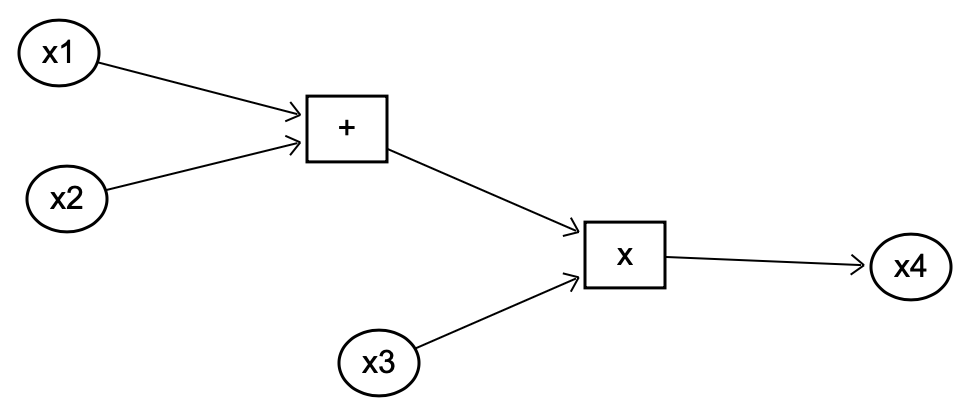
\includegraphics[width=0.7\textwidth]{graphics/arithmetic-circuit.png}
    \caption{Arithmetic circuit for computing $x_4:=x_3\cdot(x_1+x_2)$}
    \label{fig:arithmetic-circuit}
\end{figure}

In this example, $x_1$, $x_2$ and $x_3$ are input gates, $x_4$ is an output gate and there is a multiplication and an addition gate.


\section{PLONK}
\label{sec:plonk}
\subsection*{Overview}
PLONK, \textit{Permutations over Lagrange-bases for Oecumenical Noninteractive arguments of Knowledge}, was introduced by Gabizon et al. in 2019~\cite{gabizon2019plonk}. It is a zkSNARK proving system and the one that will be used and explained in this thesis.

\subsection{Constraint system}
In~\cite{gabizon2019plonk}, a constraint system $\mathcal{C}$ over $\mathbb{F}_p$ is introduced, allowing the representation of arithmetic circuits. These circuits can contain gates with at most two inputs each, and output gates that can be connected to any number of other gates.\\
Let $m$ represent the number of wires and $n$ the number of gates, excluding private input/output gates. Let $\textbf{x}\in\mathbb{F}_p^m$ be the wire assignment\footnote{A \textbf{wire assignment} referes to the assignment of specific values from the field $\mathbb{F}_p$ to the wires in an arithmetic circuit.}. Let $\textbf{a},\textbf{b},\textbf{c}\in[m]^n$ be the left, right and output vector sequence of each gate in the circuit $\mathcal{G}$, respectively. Additionally, let $\textbf{q}_\textbf{L},\textbf{q}_\textbf{R},\textbf{q}_\textbf{O},\textbf{q}_\textbf{M},\textbf{q}_\textbf{C}\in\mathbb{F}_p^n$, where each \textbf{q} term represents a selector vector\footnote{A \textbf{selector vector} is a constant used to control the behavior of the arithmetic circuit based on the type of gate being evaluated.} in $\mathbb{F}_p$ used to define constraints based on the gate type.\\
Thus, the PLONK constraint at every gate $i\in[n]$ must satisfy
\begin{equation}
    \left(\textbf{q}_\textbf{L}\right)_i\cdot\textbf{x}_{\textbf{a}_i}+ \left(\textbf{q}_\textbf{R}\right)_i\cdot\textbf{x}_{\textbf{b}_i} + \left(\textbf{q}_\textbf{O}\right)_i\cdot\textbf{x}_{\textbf{c}_i} + \left(\textbf{q}_\textbf{M}\right)_i\cdot\left(\textbf{x}_{\textbf{a}_i}\textbf{x}_{\textbf{b}_i}\right) + \left(\textbf{q}_\textbf{C}\right)_i=0
    \label{eq:plonk-constraint}
\end{equation}

For example, from the vector sequence \textbf{a}, we set $\textbf{a}_i:=j$, where $j\in[m]$ is the index of the value $\textbf{x}_j$ assigned to the left input of the $i$ gate, in other words, for each gate $i$ in the circuit, we are selecting a specific wire to be its left input.

To build a \textbf{multiplation gate} we set $\left(\textbf{q}_\textbf{L}\right)_i=0$, $\left(\textbf{q}_\textbf{R}\right)_i=0$, $\left(\textbf{q}_\textbf{M}\right)_i=1$, $\left(\textbf{q}_\textbf{O}\right)_i=-1$, $\left(\textbf{q}_\textbf{C}\right)_i=0$, and we get the following constraint for a gate $i$
\[\textbf{x}_{\textbf{a}_i}\textbf{x}_{\textbf{b}_i}-\textbf{x}_{\textbf{c}_i}=0.\]\\
Similary, for an \textbf{addition gate}, we set $\left(\textbf{q}_\textbf{L}\right)_i=1$, $\left(\textbf{q}_\textbf{R}\right)_i=1$, $\left(\textbf{q}_\textbf{M}\right)_i=0$, $\left(\textbf{q}_\textbf{O}\right)_i=-1$, $\left(\textbf{q}_\textbf{C}\right)_i=0$, resulting in the constraint:
\[\textbf{x}_{\textbf{a}_i}+\textbf{x}_{\textbf{b}_i}-\textbf{x}_{\textbf{c}_i}=0.\]\\
Lastly, for a \textbf{constant gate}, we set $\left(\textbf{q}_\textbf{L}\right)_i=1$, $\left(\textbf{q}_\textbf{R}\right)_i=0$, $\left(\textbf{q}_\textbf{M}\right)_i=0$, $\left(\textbf{q}_\textbf{O}\right)_i=0$, $\left(\textbf{q}_\textbf{C}\right)_i=-c_i$, and the corresponding constraint is
\[\textbf{x}_{\textbf{a}_i}-c_i=0.\]\\
To summarize the initial proces of PLONK: 
\begin{enumerate}
    \item We build the arithmetic circuit based on the PLONK constraint of the program, where each operation of the circuit (addition, multiplication) corresponds to a gate in the circuit.
    \item The arithmetic circuit is translated into a constraint system, formed by all the contraints used to build the circuit.
\end{enumerate}

\subsubsection*{Copy constraints}
Up until now, we have been focused on how to build gates within the arithmetic circuit. However, we are not connecting them, we are missing the wiring. Copy constraints ensure that the outputs of some gates correctly map to the inputs of subsequent gates.

\subsubsection*{Example}
Let's illustrate the PLONK protocol with an example. Consider the arithmetic circuit from Figure~\ref{fig:arithmetic-circuit-plonk}, which computes $v_4:=v_1\cdot v_2+v_3$. In this circuit, $v_1, v_2, v_3$ are private inputs (the witnesses), while $v_4$ is the public input.
\begin{figure}[htbp]
    \centering
    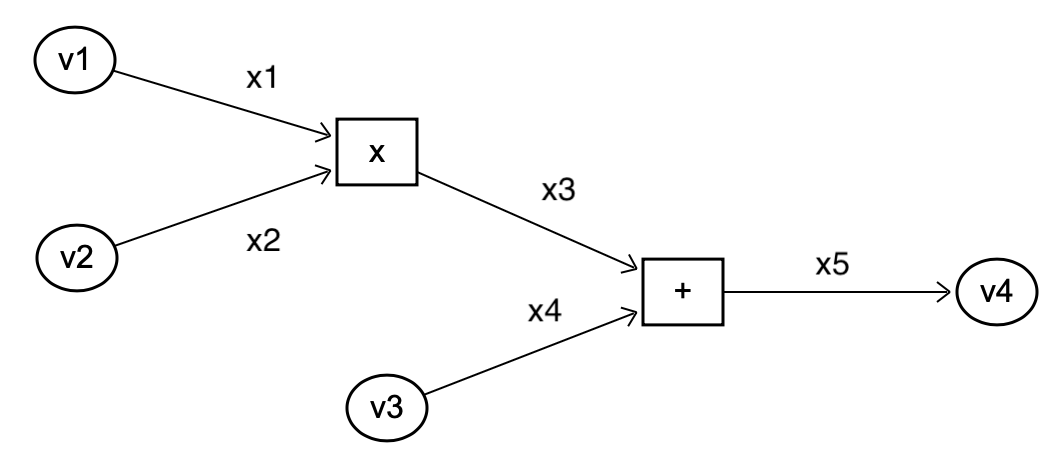
\includegraphics[width=0.7\textwidth]{graphics/arithmetic-circuit-plonk.png}
    \caption{Arithmetic circuit for computing $v_4:=v_1\cdot v_2+v_3$}
    \label{fig:arithmetic-circuit-plonk}
\end{figure}
In this arithmetic circuit we have 3 private input gates $(v_1, v_2, v_3)$, $m=5$ wires and $n=3$ gates, let $i=1$ be the multiplication gate, $i=2$ the addition gate, and $i=3$ the output gate, the sequence vectors \textbf{a}, \textbf{b}, \textbf{c }$\in[5]^3$ are\[\textbf{a}:=(1,3,5),\textbf{ b}:=(2,4,5),\textbf{ c}:=(3,5,5).\]\\
To make it more clear, let's demonstrate the process for gate $i=2$ (addition gate). The left wire $x_3=\textbf{x}_{\textbf{a}_2}$, where $\textbf{a}_2$ denotes the index of the left input wire. Similary, the right input wire $x_4=\textbf{x}_{\textbf{b}_2}$, and the output wire $x_5=\textbf{x}_{\textbf{c}_2}$, and so on for each component of the vector sequence.\\
By assigning the corresponding values to the selector vectors, depending on the type of gate as explained earlier, we get the following constraints:
\begin{align*}
    x_1\cdot x_2-x_3=0 \\
    x_3+x_4-x_5=0 \\
    x_5-v4=0
\end{align*}

Next, we need to establish the connections between different gates. In this case, it consists in connecting the multiplication gate with the addition gate and the addition with the output gate. Thus, we define the copy constraints for these cases:
\begin{align*}
    a_2=c_1 \\
    c_2=a_3
\end{align*}

\subsection{Compressing Constraints}
There is a property about polynomials, called the \textit{Schwartz-Zippel lemma}~\cite{zippel1979probabilistic, barbara2021reinforced} widely used in zero-knowledge proving systems, including Plonk. This lemma affirms that if two polynomials $P$ and $Q$ result in the same value when evaluated at some random point $a$, then it's highly probable that the two polynomials are identical.

To use this property we convert the constraint system into a polynomial expression that is true if the constraint system is satisfied.

\subsubsection*{Lagrange interpolation}
Plonk uses Lagrange interpolation to convert the constraint system to a polynomial. We define polynomials $a(i),b(i),c(i)$ to interpolate the values in \textbf{x} with the vectors \textbf{a}, \textbf{b}, \textbf{c}, and $Q_L(i),Q_R(i),Q_O(i),Q_M(i),Q_C(i)$ to interpolate $\textbf{q}_\textbf{L},\textbf{q}_\textbf{R},\textbf{q}_\textbf{O}, \textbf{q}_\textbf{M}, \textbf{q}_\textbf{C}$ for each $i$.\\
Now, using Equation~\eqref{eq:plonk-constraint} we express the constraint as a polynomial:
\begin{equation}
    Q_\text{L}(i)a(i)+Q_\text{R}(i)b(i)+Q_\text{O}(i)c(i)+Q_\text{M}a(i)b(i)+Q_\text{C}(i)=0
\end{equation}

\subsection{Polynomial commitments}
A polynomial commitment can be used to verify evaluations of a polynomial without needing access to entire polynomial itself. In other words, let's define a commitment $c$ representing the polynomial $P(x)$. There is a proof that can convince you of the value of $P(z)$ for some point $z$, without revealing the polynomial $P(x)$ itself.

The mathematical details of the polynomial commitment scheme is out of the scope of this thesis, requiring the exclusion of certain details. For a more detailed explanation look at~\cite{10.1007/978-3-642-17373-8_11}.

Intuitively, there are some equations between the polynomials that need to be checked. In Plonk, the prover need to commit to multiple polynomials. Although, the prover and the verifier could handle all the commitments one by one, in~\cite{gabizon2019plonk}, these polynomials are commited within a single step.
These commitments are evaluated at some random point $z$, along with proofs indicating that these evaluations are correct. Finally, the equations are applied to these evaluations rather than the original polynomials.\\
Thus, the final proof is just some commitments and the evaluations, and can be checked with a few equations.

\chapter{State of the Art on Zero-Knowledge Friendly Hash Functions}
\label{sec:zk-hashes}
This chapter will provide a theoretical approach of the hash functions that will be implemented.

\section*{Overview}
Most of the hash functions that work in zero-knowledge operate within a finite field, with their efficiency usually related to the number of multiplications and additions in the circuit.
Traditional hash functions such as SHA-256 or AES are designed to operate on bits and perform bitwise operations. However, when these bit-oriented hash functions are used in zero-knowledge proofs, they often result in very large circuit sizes, reducing efficiency. This inefficiency is due to the need for representing bitwise operations of long bit-size numbers, which usually involve numerous multiplications and additions within the circuit.

To address these issues, Arithmetization-Oriented (AO) hash functions have been developed. These hash functions are designed specifically for zero-knowledge proofs and operate within a finite field. By focusing on arithmetic operations rather than bitwise operations, AO hash functions simplify the circuit complexity. Consequently, they enable more efficient computations in zero-knowledge proofs.

Moreover, some techniques will be introduced to minimize the number of multiplications in the zero-knowledge circuits for better efficiency.


\section{MiMC}
The first hash funcion we explain is MiMC~\cite{albrecht2016mimc}, it was publiched by Albrecht et al. in 2016 and designed to provide high performance for the applications of zero-knowledge proofs, Fully-Homomorphic Encryption (FHE) and Multi-Party-Computation (MPC) frameworks. This hash function is very simple, its core non-linear component is the function $F(x) := x^3$ that is iterated with subkey additions. The advantatge of using this function is that only requires two field multiplications, in contrast to using a look-up table S-box, which can be expensive to represent in an arithmetic circuit, for example.\\
MiMC provides three cryptographic primitives. First, we are going to describe the block cipher and finally a permutation. We consider MiMC just for cipher/permutation, and GMiMC~\cite{cryptoeprint:2019/397} or Hades~\cite{10.1007/978-3-030-45724-2_23} for hashing. All these primitives work in a finite field $\mathbb{F}_q$, where $q$ is a prime $p$ or a power of 2. In this thesis we will focus on $q=p$.

\subsection*{Block cipher}
First of all we are going to explain the block cipher, MiMC-$b/k$ is a keyed permutation where each input block is maped to a unique output block with $b$ as block size and $k$ as key size.

\subsubsection*{MiMC-p/p}
The MiMC block cipher takes an input $x \in F_{p}$ and does $r$ iterations over a round function. The round function consists on a key addition of the $k$ vector, the addition of a round constant $c_i \in F_{p}$ and the previous discussed non-linear function $F(x) := x^d$ for $x \in F_{p}$ is applied for updating the current sate. Additionally, we need to assure that $d\geq3$ is the smallest
permutation, so gcd$(d,p-1)=1$, explained in section~\ref{sec:s-box}.\\
The encryption function consists in $r$ iterations over the round functions, adding the key $k$ after $r$ rounds have been performed.\\
So, the round function is defined as 
\begin{equation}
    F_i(x) = F\left(x \oplus k \oplus c_i\right)
\end{equation}
and the encryption function is expressed as
\begin{equation}
    E_k(x) = \left(F_{r-1} \circ F_{r-2} \circ \dots F_0\right)(x) \oplus k
\end{equation}

Figure~\ref{fig:mimc-enc-img} represents the encryption process of MiMC for $d=3$.

The equation for calculating the number of rounds is
\begin{equation}
    r = \left\lceil\frac{p}{\log_2 3}\right\rceil
\end{equation}

The values of the $r - 1$ round constants can be choosen randomly from the field $\mathbb{F}_{p}$ except for the first $c_0$ and last $c_r$ round constant whose values are 0.

\begin{figure}[h]
    \centering
    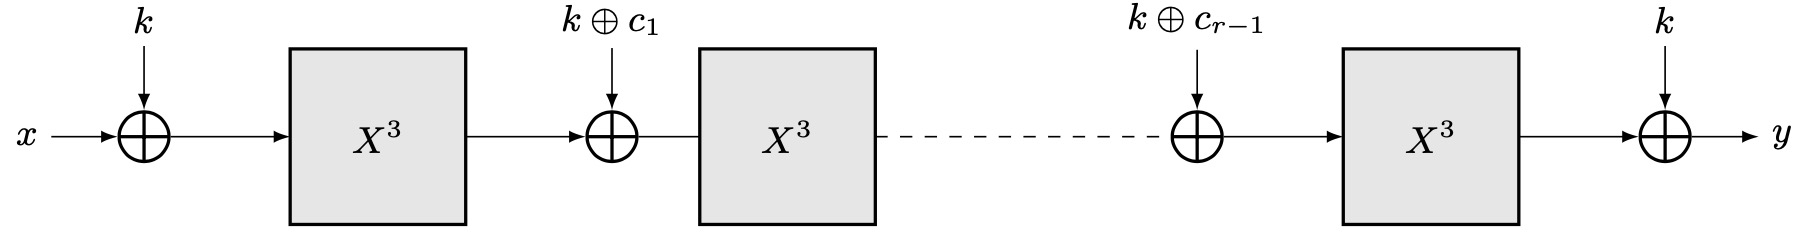
\includegraphics[width=\textwidth]{graphics/enc_mimc.jpg}
    \caption{Encryption process of MiMC~\cite{albrecht2016mimc} for $d=3$}
    \label{fig:mimc-enc-img}
\end{figure}

\subsubsection*{MiMC-2p/p}
In addition to the standard version of MiMC, there are some other variants, including those using a Feistel network, with extended key size, and using different round functions.
We focus on the \textbf{Feistel network} variant over prime fields, MiMC-$2p/p$. By using the Feistel network in the block cipher, we can process larger blocks, with two blocks being processed in each round.\\ 
The new round function of MiMC-$2p/p$ differs from the one in MiMC-$p/p$, taking the form~\cite{albrecht2016mimc}:
\begin{equation}
    x_L\|x_R \longleftarrow x_R \oplus \left(x_L \oplus k \oplus c_i\right)^3\|x_L
\end{equation}
However, the encryption function is the same as in MiMC-$n/n$.\\
In the Feistel network the round constants $c_i$ are also randomly generated from the $\mathbb{F}_{p}$ field. The cost for processing larger blocks comes with the incress of the number of rounds, where

\begin{equation}
    r' = 2 \cdot r = 2 \cdot \left\lceil\frac{p}{\log_2 3}\right\rceil
\end{equation}

Here, $r$ is the number of rounds of MiMC-$p/p$. Figure~\ref{fig:feistel-network} represents the encryption process of MiMC-$2p/p$. Because there is one more XOR operation and the number of rounds needs to be doubled, the computation of the encryption will be slightly slower than the regular MiMC.

\begin{figure}[htbp]
    \centering
    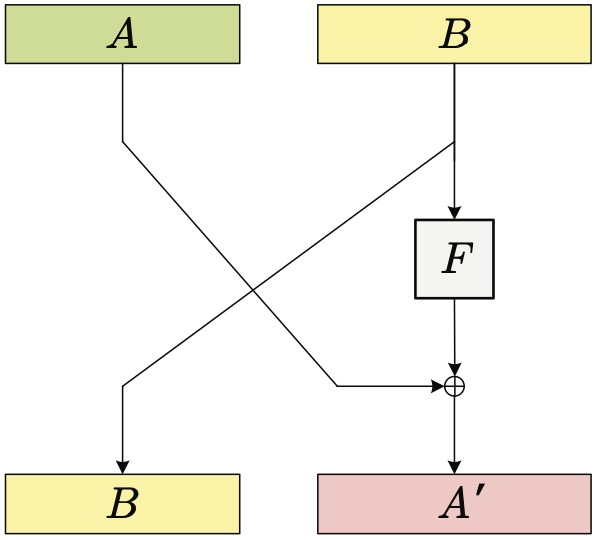
\includegraphics[width=0.4\textwidth]{graphics/feistel.jpg}
    \caption{Feistel network}
    \label{fig:feistel-network}
\end{figure}

\subsection*{MiMC permutation}
The MiMC permutation, MiMC$^P$, is obtained by setting all the key $k$ values to 0.

\section{Poseidon}
\label{sec:poseidon}
The Poseidon hash function~\cite{grassi2021poseidon}, published by Grassi et al. in 2021 works using the Poseidon$^\pi$ permutation within the sponge framework. This permutation is based on the Hades design, which will be explained below.
The hash function takes inputs from the $\mathbb{F}_{p}$ field, where $p$ is a prime number, and maps them to a fixed-length output over the $\mathbb{F}_{p}$ field, $\mathbb{F}_{p}^*\longrightarrow\mathbb{F}_{p}^o$, with $o$ representing the length of the output.

\subsection*{Hades strategy}
The Hades strategy doesn't use $r$ number of rounds, instead, it uses $r_f$ rounds initially, with full S-box layers. Subsequently, after these $r_f$ rounds, $r_p$ rounds are applied, but with only a single S-box. Finally $r_f$ rounds are applied again at the end, using full S-box layers.

Figure~\ref{fig:hades-enc-img} represents this explained aproach.\\
\begin{figure}[htbp]
    \centering
    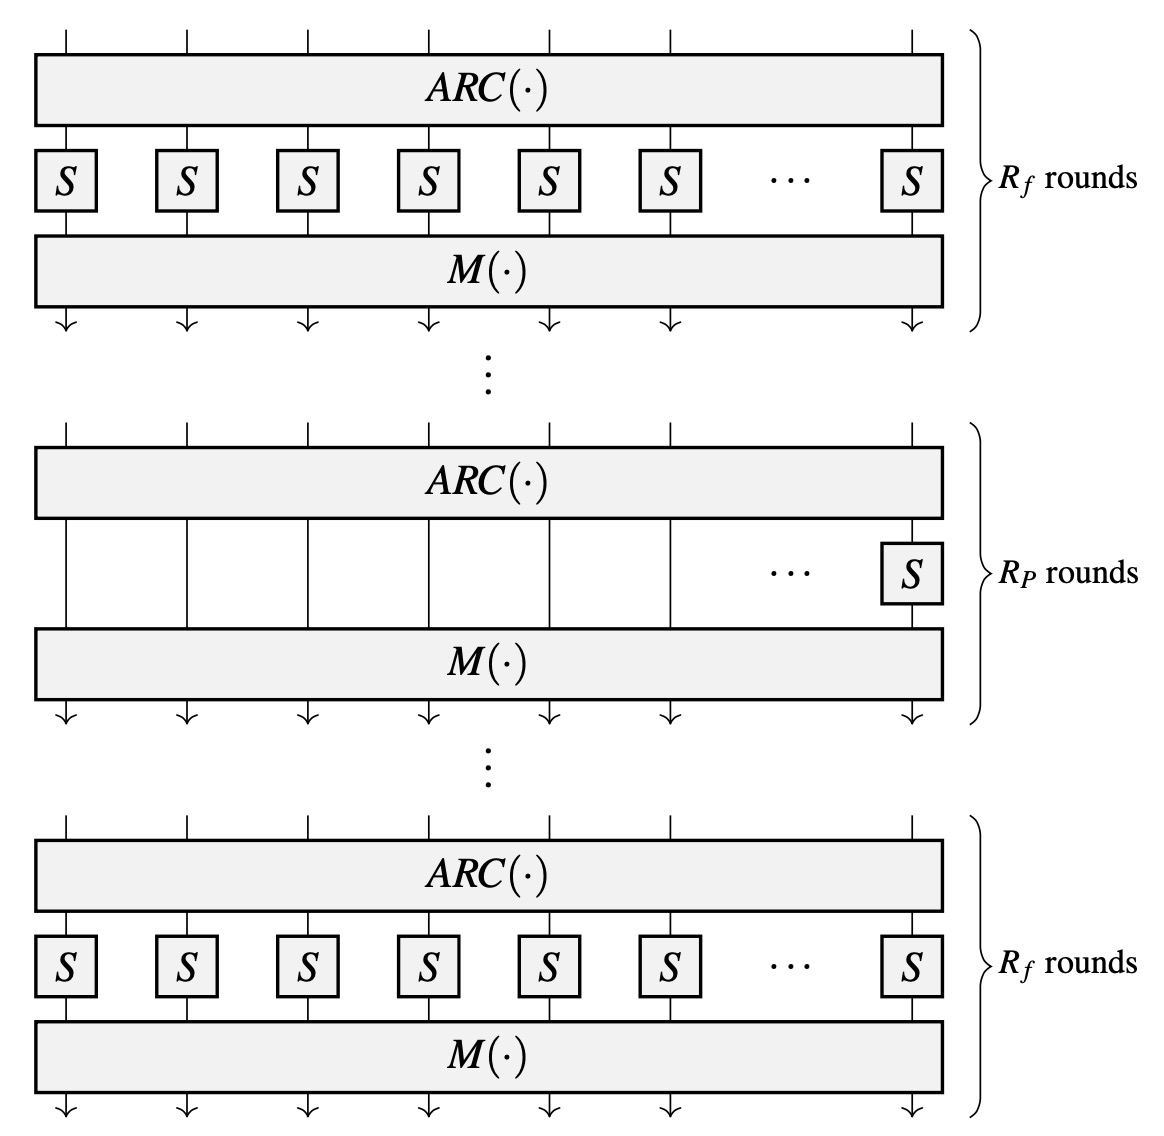
\includegraphics[width=0.8\textwidth]{graphics/hades_enc.jpg}
    \caption{Encryption process of Hades~\cite{grassi2021poseidon}}
    \label{fig:hades-enc-img}
\end{figure}

\subsubsection*{Poseidon round function}
The Poseidon round function is composed of two different rounds: full rounds and partial rounds.
The full round $\mathcal{E}$ is defined as
\begin{equation}
    \mathcal{E}_i(x) = M\cdot\left(\left(x_0+c_0^{(i)}\right)^d,\dots,\left(x_{t-1}+c_{t-1}^{(i)}\right)^d\right)
\end{equation}
for $i \in \{0,1,\dots,R_{r_f}-1\}$. The partial round $\mathcal{I}$ is defined as
\begin{equation}
    \mathcal{I}_i(x) = M\cdot\left(\left(x_0+c_0^{(i)}\right)^d,x_1+c_1^{(i)},\dots,x_{t-1}+c_{t-c}^{(i)}\right)
\end{equation}

for $i \in \{0,1,\dots,R_{r_p}-1\}$.

Table~\ref{tab:pos-round} represents the three steps of one round of Poseidon$^\pi$
\begin{table}[htbp]
    \centering
    \begin{tabular}{rl}
        \toprule
        & Hades round function \\
        \midrule
        1 & Add the round constants, denotated by $ARC(\cdot)$ \\
        2 & Apply substitution \\
        & i.  Full S-box$(\cdot)$ for $r_f$ rounds \\
        & ii. Partial S-box$(\cdot)$ for $r_p$ rounds \\
        3 & Multiply state with the MDS matrix, denotated by $M(\cdot)$ \\
    \end{tabular}
    \caption{One round of the Poseion$^\pi$}
    \label{tab:pos-round}
\end{table}

Next, we will describe the components of the Poseidon round function.

\subsubsection*{Constant layer}
The ARC($\cdot$) consists in adding the round constants $c_i$ to the state, where each component of the state will have a round constant added.

\subsubsection*{S-box layer}
The s-box layer is defined as Sbox$(x) = x^d$, where $d \geq 3$ is the smallest integer that satisfies $gcd(d,p-1) = 1$. For rounds without an S-box ($r_p$ rounds), the state remains unchanged and is forwarded as it is to the next round.

\subsubsection*{Linear layer}
The $t\times t$ Matrix with elements in $\mathbb{F}_{p}$ is a Maximum Distance Separable (MDS) matrix, which guarantees that each state component depends on each other component in each round. All $t$ components of the state will be multiplied by the $t \times t$ MDS matrix. The result of this multiplications is the input state for the next round layer. Unlike the Hades strategy, the linear layer is omitted in the last round.

\subsection*{Poseidon permutation}
The Poseidon$^\pi$ permutation over the vector space $\mathbb{F}_p^t$, where $t \geq 2$ is the length of the sponge state, is defined by
\begin{equation}
    \mathcal{P}(x) = \mathcal{E}_{R_F-1} \circ \dots \circ \mathcal{E}_{R_F/2} \circ \mathcal{I}_{R_P-1} \circ \dots \circ \mathcal{I}_0 \circ \mathcal{E}_{R_F/{2-1}} \circ \dots \circ \mathcal{E}_0(x),
\end{equation}
\label{eq:poseidon-perm}
where $\mathcal{E}$ represents a full round of the $R_F$ rounds and $\mathcal{I}$ is a partial round of $r_P$ rounds, with $R_F = 2\cdot r_f$.

\subsection*{Poseidon hash}
The Poseidon hash operates within the sponge construction, in the vector space $\mathbb{F}_p^{r+c}$, where $r$ is the rate and $c$ is the capacity of the sponge.

\section{Poseidon2}
The Poseidon2 hash function~\cite{grassi2023poseidon2} published by Grassi et al. in 2023, works within the sponge construction, being a more efficient version of Poseidon$^\pi$. Below, we explain the Poseidon2 hash, the Poseidon2 permutation and his round function.

\subsection*{Poseidon2 round function}
Similar to Poseidon, the Poseidon2 round function consists on two different rounds, a full round and a partial round.\\
The full round, $\mathcal{E}$, is defined as
\begin{equation}
    \mathcal{E}_i(x) = M_{\mathcal{E}}\cdot\left(\left(x_0+c_0^{(i)}\right)^d,\left(x_1+c_1^{(i)}\right)^d,\dots,\left(x_{t-1}+c_{t-c}^{(i)}\right)^d\right)
\end{equation}
where $d$ is the exponent of the S-box, and $c_j^{(i)}$ the j-th round constant in the i-th full round.\\
The partial round $\mathcal{I}$ is defined as
\begin{equation}
    \mathcal{I}_i(x) = M_{\mathcal{I}}\cdot\left(\left(x_0+\hat{c_0}^{(i)}\right)^d,x_1,\dots,\left(x_{t-1}\right)\right)
\end{equation}
where $d$ is the same exponent as before, and $\hat{c}_0^{(i)}$ is the round constant in the i-th partial round.\\
A description of the components used in the Poseidon2 round function is provided below.

\subsubsection*{Constant layer}
The round constants are generated as in Poseidon$^\pi$.

\subsubsection*{Linear layer}
Firstly, the case of $t = 4t' \geq 4$ is considered, followed by $t\in\{2,3\}$.
For the \textbf{full rounds} and $t = 4t'$ with $t' \in \mathbb{N}$, the matrix is defined as
\begin{equation}
    M_\mathcal{E} =
    \begin{cases}
        M_4 & \text{if } t=4, \\
        \text{circ}\left(2\cdot M_4,M_4,\dots,M_4\right)\in \mathbb{F}_p^{t\times t} & \text{if } t\geq 8,
    \end{cases}
\end{equation}
where $M_4$ is a $4\times 4$ MDS matrix
\begin{equation}
    M_4 = 
    \begin{pmatrix}
        5 & 7 & 1 & 3 \\
        4 & 6 & 1 & 1 \\
        1 & 3 & 5 & 7 \\
        1 & 1 & 4 & 6
    \end{pmatrix}
    ,
\end{equation}

An efficient way for computing vector per matrix multiplication is defined in~\cite{duval2018mds}. Corresponding to the $M_{4,4}^{8,4}$ matrix, with $\alpha = 2$.

For the \textbf{partial rounds}, the MDS matrix is no longer necessary. In this case, the matrix $M_\mathcal{I}$ is defined as
\begin{equation}
    M_{\mathcal{I}} = 
    \begin{pmatrix}
        \mu_0 & 1 & \dots & 1 \\
        1 & \mu_1 & \dots & 1 \\
        \vdots & \vdots & \ddots & \vdots \\
        1 & 1 & \dots & \mu_{t-1}
    \end{pmatrix}
    ,
\end{equation}

where $\left(\mu_0,\mu_1,\dots,\mu_{t-1}\right)$ are random elements from the field $\mathbb{F_p}\backslash\{0,1\}$.

\subsubsection*{Plonk Arithmetization}
For the partial round vector per matrix multiplication. Let's define a vector $\left(x_0,x_1,\dots x_{t-1}\right)$, the computation of the multiplication is
\begin{equation}
    \begin{cases}
        s = x_0,x_1,\dots ,x_{t-1}, \\
        y_i = \left(\mu_i-1\right)x_i+s & \text{for }i\in \{0,1,\dots,t-1\},
    \end{cases}
\end{equation}
where $s$ represents the sum of the elements of the vector and $y$ is the output vector.\\
Additionally, for $t\in\{2,3\}$, we set the condition that $M_\mathcal{I}$ is MDS, so, first $M_{\mathcal{I}}$ is computed and we set $M_{\mathcal{I}} = M_{\mathcal{E}}$. Appart from this we also check for
\begin{itemize}
    \item $t=2$ if $\mu_0\mu_1-1 \neq 0$ and $\mu_0,\mu_1 \neq 0$,
    \item $t=3$ if $\mu_0\mu_1\mu_2-\mu_0-\mu_1-\mu_2 \neq 0$ and
        $\mu_0\mu_1\mu_2\neq0,$  $\mu_0\mu_1-1\neq0,$ $\mu_0\mu_2-1\neq0,$ $\mu_1\mu_2\neq0$.
\end{itemize}

\subsubsection*{S-box layer}
The S-box layer is defined as Sbox$(x) = x^d$, where $d\geq3$ is the smallest positive integer such that gcd$\left(d,p-1\right)=1$.

\subsection*{Poseidon2 permutation}
The permutation is defined over the $\mathbb{F}_p^t$ vector space, where $p$ is a prime number and $t \in \{2,3,4,\dots,4\cdot t',\dots,24\}$ is the length of the state of the sponge for $t' \in \mathbb{N}$. The Poseidon2$^\pi$ is defined as
\begin{equation}
    \mathcal{P}_2(x) = \mathcal{E}_{R_F-1} \circ \dots \circ \mathcal{E}_{R_F/2} \circ \mathcal{I}_{R_P-1} \circ \dots \circ \mathcal{I}_0 \circ \mathcal{E}_{R_F/{2-1}} \circ \dots \circ \mathcal{E}_0(M_{\mathcal{E}\cdot}x)
\end{equation}
where $\mathcal{E}$ is the full round and $\mathcal{I}$ is the partial round, whith the same number of rounds as in Equation~\ref{eq:poseidon-perm} of Poseidon$^\pi$.

\subsection*{Poseidon2 hash}
Similar to the other hash functions presented in this thesis, the Poseidon2 hash also operates within a sponge construction in the field $\mathbb{F}_p^{r+c}$, where $r$ is the rate and $c$ the capacity of the sponge.

\subsection*{Poseidon$^\pi$ vs Poseidon2$^\pi$}
The differences between the permutation of Poseidon2 and Poseidon are provided below. Figure~\ref{fig:poseidon-vs-2} shows a visual representation of these difference.
\begin{itemize}
    \item The linear layer is also applied at the input of the permutation.
    \item Two diferent linear layers are used for $t\geq4$.
    \item In each round only one round function is applied.
\end{itemize}

\begin{figure}[htbp]
    \centering
    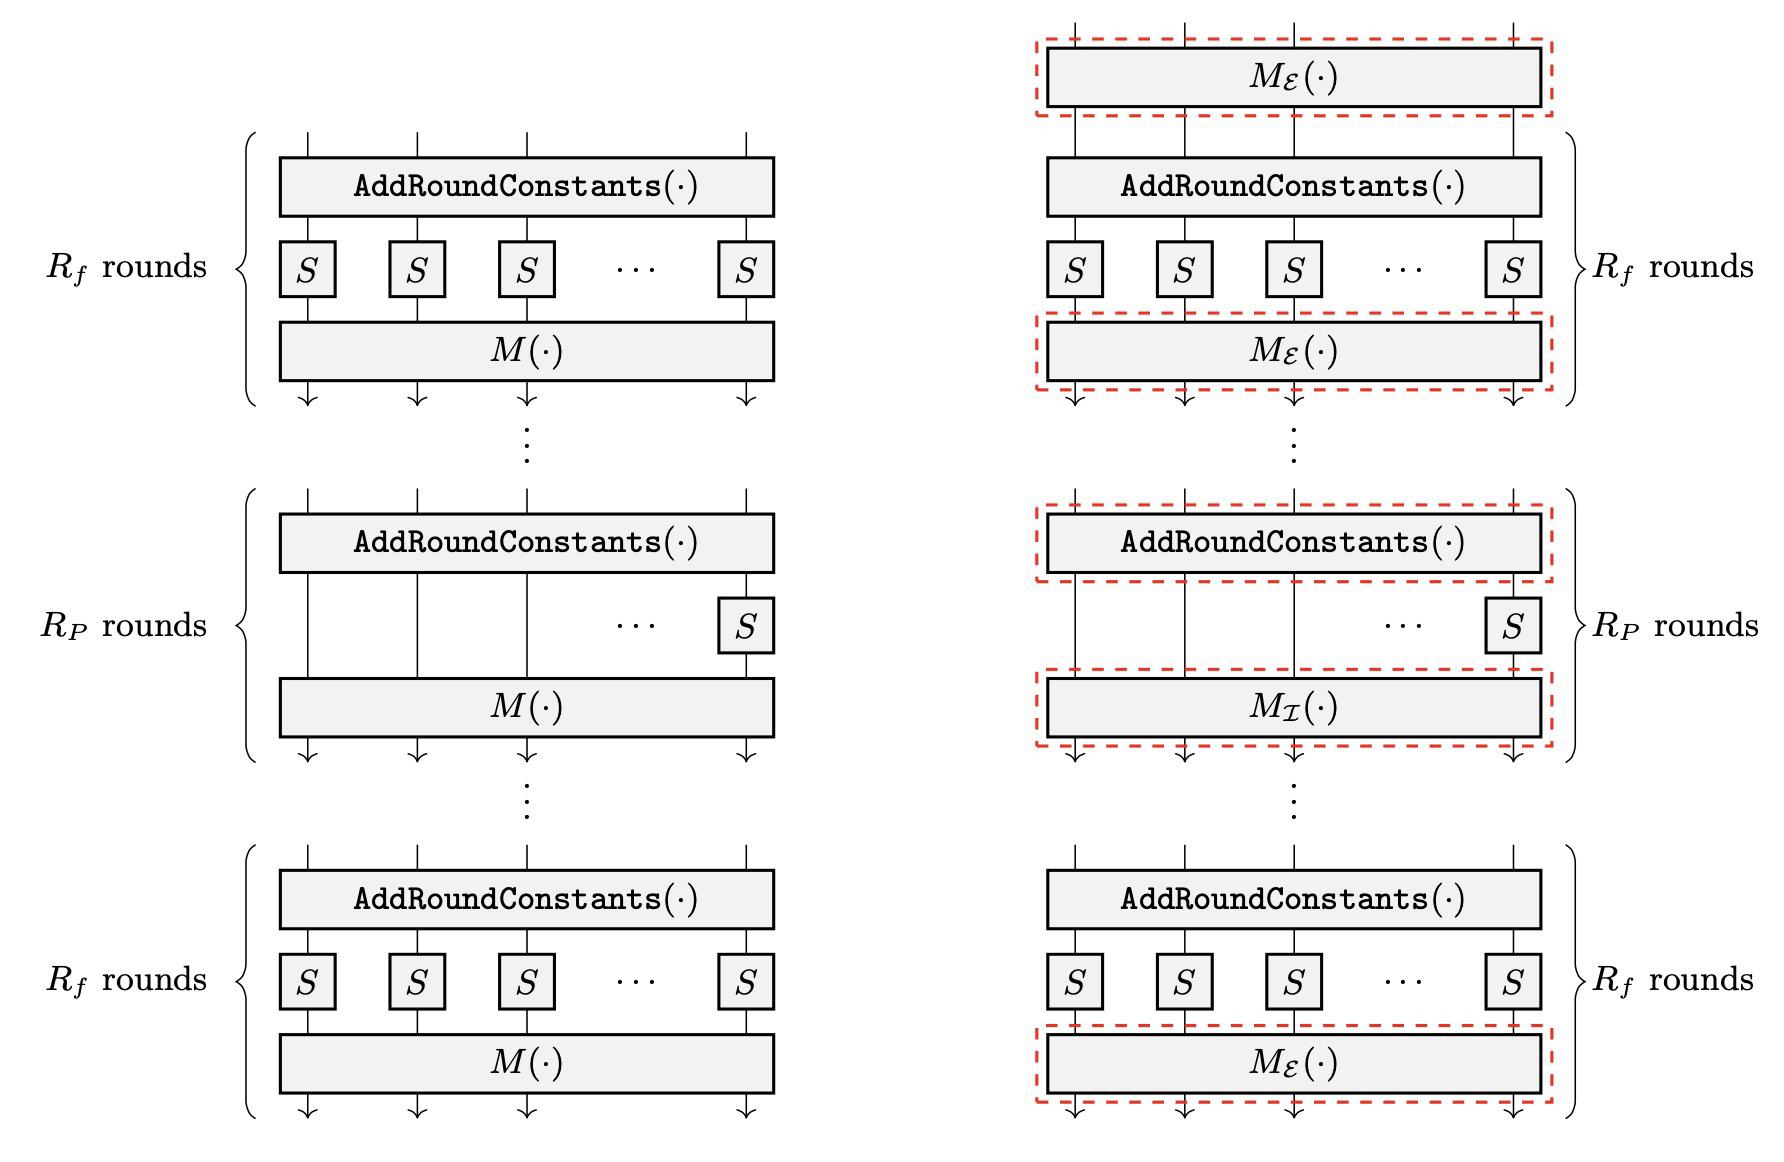
\includegraphics[width=\textwidth]{graphics/poseidon_vs_poseidon2.png}
    \caption{Poseidon$^\pi$ vs Poseidon2$^\pi$~\cite{grassi2023poseidon2}}
    \label{fig:poseidon-vs-2}
\end{figure}

\section{Rescue-prime}
\label{sec:Rescue-prime}
Rescue~\cite{szepieniec2020rescue} published by Szepieniec et al. in 2020, operates on field elements on $\mathbb{F}_{p}$, where $p$ is a prime field, and the state is a vector in the vector space $\mathbb{F}_{p}^m$, where $m$ is the number of elements. Here, we will explain both the standard and the optimized versions of Rescue-prime.

\subsection*{Rescue round function}
The Rescue round function~\cite{aly2020design} operates over the vector space $\mathbb{F}_p^{m}$, where $p$ is a prime number.
Below, Table~\ref{tab:rescue-sing-round} presents the components and steps of a single round $i$, while Figure~\ref{fig:rescue-i-round} provides a diagram of it.


\begin{table}[htbp]
    \centering
    \begin{tabular}{rl}
        \toprule
        & Rescue round function \\
        \midrule
        1 & S-box layer, apply $(\cdot)$ to each element of the state. \\
        2 & Linear layer, matrix-vector multiplication of the MDS matrix and the state. \\
        3 & Constants layer, add from the list of round constants $\{C_i\}_{i=0}^{2mN-1}$, $m$ constants \\
        & to the state. \\
        4 & Inverse S-box layer, apply $(\cdot)^{\alpha^{-1}}$ to each element of the state. \\
        5 & Liner layer, matrix-vector multiplication of the MDS matrix and the state. \\
        6 & Constants layer, add from the list of round constants $\{C_i\}_{i=0}^{2mN-1}$, $m$ constants \\
        & to the state. \\
    \end{tabular}
    \caption{One round components}
    \label{tab:rescue-sing-round}
\end{table}

\begin{figure}
    \centering
    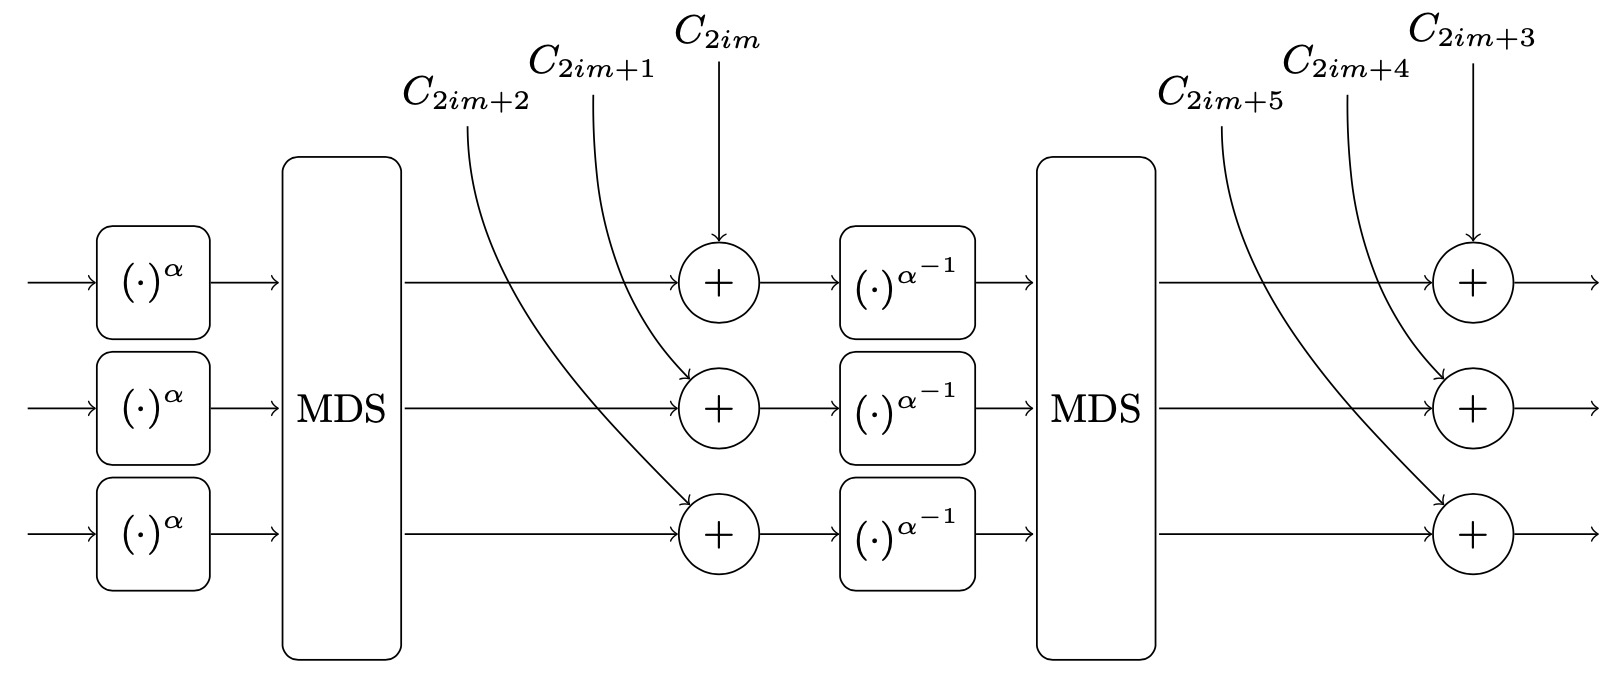
\includegraphics[width=0.9\textwidth]{graphics/rescue_i_round.jpg}
    \caption{Round $i$ of Rescue$^\pi$~\cite{szepieniec2020rescue}}
    \label{fig:rescue-i-round}
\end{figure}

To build the S-box, we find the smallest prime $\alpha$ such that $gcd(p-1, \alpha) = 1$. Therefore, the S-box is defined as $S : \mathbb{F}_{p} \longrightarrow \mathbb{F}_{p} : x \mapsto x^\alpha$ and $S^{-1} : \mathbb{F}_{p} \longrightarrow \mathbb{F}_{p} : x \mapsto x^{1/\alpha}$, where $1/\alpha$ is the multplicative inverse of a modulo $p-1$, whose existance is guaranteed by the fact that gcd$(\alpha, p - 1) = 1$. The generation of the MDS matrix and the round constants is out of the scope of this thesis, although~\cite{szepieniec2020rescue} provides a SageMath implementation with the computation of the number of rounds and the MDS matrix.

\subsection*{Rescue-prime optimized}
The optimized version of the Rescue-prime~\cite{ashur2022rescue} published in 2022, works only over the Goldilocks prime field, where $p = 2^{64} - 2^{32} + 1$, explained in section~\ref{sec:finite-fields}.

It uses the same components of the standard Rescue-prime round function, but the order of the operations differs from the standard version. The new order is presented in Table~\ref{tab:rescue-opt-round-comp}. 

\begin{table}[htbp]
    \centering
    \begin{tabular}{rl}
        \toprule
        & Rescue-prime optimized round function \\
        \midrule
        1 & MDS matrix \\
        2 & Constant layer \\
        3 & S-box layer \\
        4 & MDS matrix \\
        5 & Constant layer \\
        6 & Inverse S-box layer \\
        \bottomrule
    \end{tabular}
    \caption{Rescue-prime optimized single round components}
    \label{tab:rescue-opt-round-comp}
\end{table}

\subsubsection*{Parameters}
In the optimized version, certain parameters are fixed. The exponents of the S-box and the inverse S-box, $\alpha$ and $\alpha^{-1}$, are set to $\alpha = 7$ and $\alpha^{-1} = 10540996611094048183$. Table~\ref{tab:rescue-param-opt} provides additional parameters.

\begin{table}[htbp]
    \centering
    \begin{tabular}{cccc}
      \toprule
      Prime field $p$ & $2^{64} - 2^{32} + 1$  \\
      Number of rounds $N$  & 7   \\
      State size $m$       & 12   \\
      Rate $r$       & 8          \\
      Capacity $c$  & 4           \\
      \bottomrule
    \end{tabular}
    \caption{Integer parameters for the Rescue-prime optimization}
    \label{tab:rescue-param-opt}
  \end{table}

  \subsubsection*{MDS Matrix}
The MDS matrix is a circulant matrix with the first row defined as:
\[[7,23,8,26,13,10,9,7,6,22,21,8]\]

\subsubsection*{Overwrite mode}
In contrast to the standard Sponge construction, the elements from the state associated with the rate are added by the matching elements from the input chunk, but in this optimized case, the elements are not added but they are overwritten. In other words, if the $state[j]$ represents the state elements and $input[j]$ the input chunk, it will permorm this absorbing operation $state[j] \leftarrow input[j]$ instead of $state[j] \leftarrow state[j] + input[j]$ 

\subsubsection*{Indexing of state elements}
In the optimized version, the state is composed by the capacity and the rate, where each one indices from 0 to $c - 1$ and $c$ to $m - 1$, respectively.

\subsection*{Rescue-prime permutation}
The Rescue-prime permutation consists in iterating N times the round function.

\subsection*{Rescue-prime hash}
Both the standard and optimized versions of Rescue-prime utilize the Sponge construction for hashing.

\subsubsection*{Sponge construction}
There is a modification in the squeezing phase of the sponge construction and the one explained in section~\ref{sec:sponge-construction}. In the squeezing phase the top $r$ elements of the state are the output, note that we don't apply the permutation in this phase.

Figure~\ref{fig:rescue-prime-hash} demonstrate this modification for $N=2$.

\begin{figure}
    \centering
    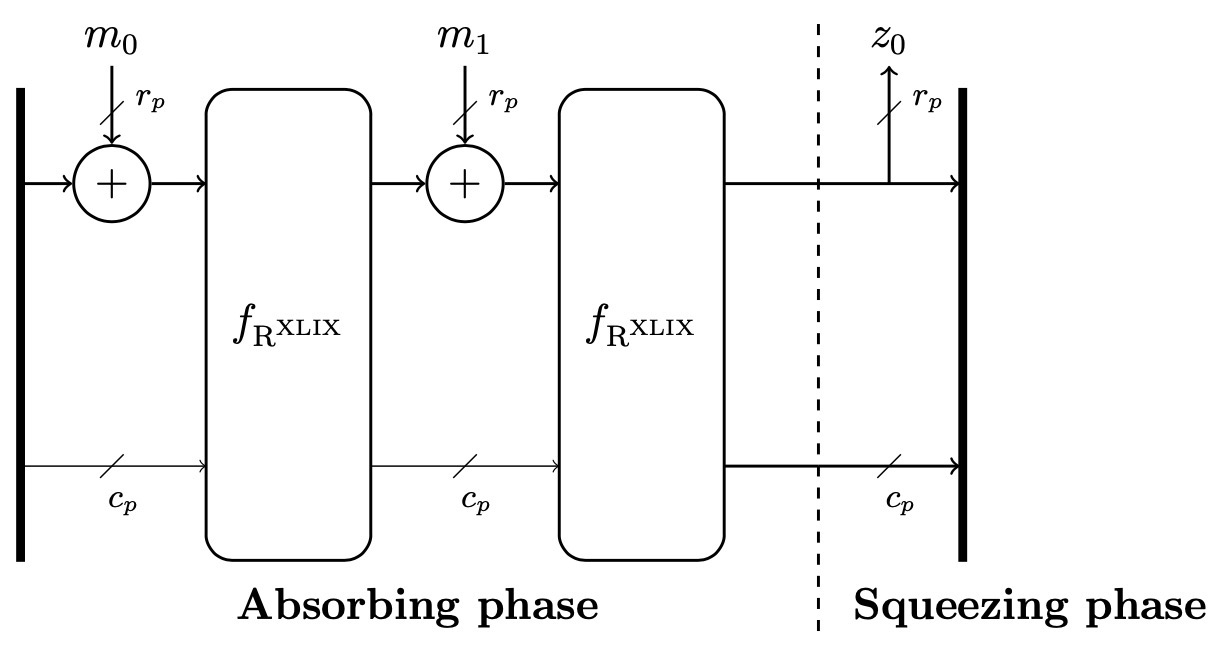
\includegraphics[width=0.7\textwidth]{graphics/rescue-prime-hash.png}
    \caption{Rescue-prime hash function with $N=2$~\cite{szepieniec2020rescue}}
    \label{fig:rescue-prime-hash}
\end{figure}

\section{Griffin}
\label{sec:griffin}
We are going to explain the Griffin hash function~\cite{grassi2022horst}, proposed by Grassi et al. in 2022. It is a hash function that operates over the permutation, Griffin$^\pi$, and a round function.

\subsection*{Griffin round function}
The Griffin round function, denoted as $\mathcal{F}_i$, is defined as
\begin{equation}
    \mathcal{F}_i(\cdot) = c^{(i)} + \mathcal{M} \times \mathcal{S}(\cdot).
\end{equation}
Here, $c^{(i)} \in \mathbb{F}_{p}^t$ is the round constant, where $c^{R-1} = 0$, $\mathcal{S} : \mathbb{F}_{p}^t \longrightarrow \mathbb{F}_{p}^t$ is a nonlinear layer, and $i \in \{0,1,\dots,R-1\}$ with $R$ being the number of rounds. The round constants that are added to the state will be different in every round but the matrix $M$ that is applied to the state will be the same in every round.\\
Each one of the components of the round function will be explained next.

\subsubsection*{Nonlinear layer \textit{S}}
The permutation is limited in $t \leq 24$, with $d$ taking values from $\{3,5,7,11\}$, similar to the previous hash functions. These values are choosen such that $gcd(d,p-1) = 1$. Additionally, $\alpha_i$ and $\beta_i \in \mathbb{F}_{p}^2 \backslash\{(0,0)\}$ are a pairwise distinct, ensuring that $\alpha_i^2 - 4\beta_i$ is a quadratic nonresidu modulo $p$ for $2\leq i \leq t-1$.\\
The nonlinear layer $\mathcal{S}(x_0,\dots,x_{t-1}) = y_0 \| \cdot\cdot\cdot\|y_{t-1}$ is composed of two nonlinear sublayers defined via three different nonlinear functions. Two of them are defined via the invertible power maps $x\mapsto x^d$ and $x\mapsto x^{1/d}$, inspired by Rescue. The final one uses the Horst scheme (Section~\ref{sec:horst}), using the map $(x,y)\mapsto(x,y\cdot G(x))$ for a quadratic function $G$ such that $G(z)\neq0$ for each $z$. It is defined as:
\begin{equation}
    y_i = \begin{cases}
        x_0^{1/d} & \text{if i } = 0, \\
        x_1^d & \text{if i } = 1, \\
        x_2 \cdot \left(\left(L_i\left(y_0,y_1,0\right)\right)^2 + \alpha_2 \cdot L_i\left(y_0,y_1,0\right)+ \beta_2\right) & \text{if i } = 2, \\
        x_i \cdot \left(\left(L_i\left(y_0,y_1,x_{i-1}\right)\right)^2 + \alpha_i \cdot L_i\left(y_0,y_1,x_{i-1}\right) + \beta_i\right) & \text{otherwise},  
    \end{cases}
\end{equation}
where $L_i : \mathbb{F}_{p}^3 \longrightarrow \mathbb{F}_{p}$ represents $L_i\left(z_0,z_1,z_2\right) = \gamma_i \cdot z_0 + z_1 + z_2$ for $\gamma_i \in \mathbb{F}_{p} \backslash \{0\}$.

\textbf{Linear layer \textit{M}}\\
For $t \in \{3,4\}$, the matrix $M$ must be MDS,
\begin{equation}
    M_3 = 
    \begin{pmatrix}
        2 & 1 & 1 \\
        1 & 2 & 1 \\
        1 & 1 & 2 
    \end{pmatrix}
    \text{, } M_4 = 
    \begin{pmatrix}
        5 & 7 & 1 & 3 \\
        4 & 6 & 1 & 1 \\
        1 & 3 & 5 & 7 \\
        1 & 1 & 4 & 6
    \end{pmatrix}
    \text{,}
\end{equation}

we can use the efficient method proposed in~\cite{duval2018mds} to compute the matrix per vector multiplication, where the $M_4$ corresponds to $M_{4,4}^{8,4}$, setting $\alpha = 2$.

When $t \geq 8$, $M$ is
\begin{equation}
    M = M'' \times M' \equiv M' \times M'' =
    \begin{pmatrix}
        2\cdot M_4 & M_4 & \dots & M_4 \\
        M_4 & 2\cdot M_4 & \dots & M_4 \\
        \vdots & \vdots & \ddots & \vdots \\
        M_4 & M_4 & \dots & 2\cdot M_4
    \end{pmatrix}
    ,
\end{equation}
where $M'=$ diag$\left(M_4,M_4,\dots,M_4\right) \in \mathbb{F}_{p}^{t\times t}$ and $M'' =$ circ$\left(2\cdot I, I,\dots,i\in \mathbb{F}_{p}^{t\times t}\right)$ and $M_4$ is a $4\times 4$ MDS matrix and $I$ is the $4\times 4$ identity matrix.

\subsection*{Griffin permutation}
The Griffin permutation, denotated as $\mathcal{G}^\pi : \mathbb{F}_{p}^t \longrightarrow \mathbb{F}_{p}^t$ is defined as
\begin{equation}
    \mathcal{G}^\pi(\cdot) := \mathcal{F}_{\mathcal{R}-1} \circ \mathcal{F}_1 \circ \mathcal{F}_0(\mathcal{M}\times \cdot),
\end{equation}
where $\mathcal{M}$ is a matrix defined as above, and $\mathcal{F}_i : \mathbb{F}_{p}^t \longrightarrow \mathbb{F}_{p}^t$ represents the round function of the $\mathcal{G}^\pi$ permutation.\\
Figure~\ref{fig:griffin-permutation} shows the $\mathcal{G}^\pi$ permutation, where $\boxplus$ represents the addition opeeration of two vectors in the field $\mathbb{F}_{p}^t$.

\subsection*{Griffin-Sponge hash function}
The Griffin hash function operates over a field $\mathbb{F}_{p}$, where $p$ is a prime number and $t\in \{3,4t'\}$ the length of the state for a positive integer $t' \in \{1,2,\dots,6\}$, that means that $t$ must be 3 or a multiple of 4. Additionally, due to the use of the sponge construction, the rate $r$ must satisfy $r \geq t/3$.\\
Figure~\ref{fig:griffin-hash} provides the Griffin-Sponge hash function, where $\oplus$ represents the addition operation of two vectors in the field $\mathbb{F}_{p}^r$ and $\mathcal{G}^\pi$ the Griffin permutation.

\begin{figure}[htbp]
    \centering
    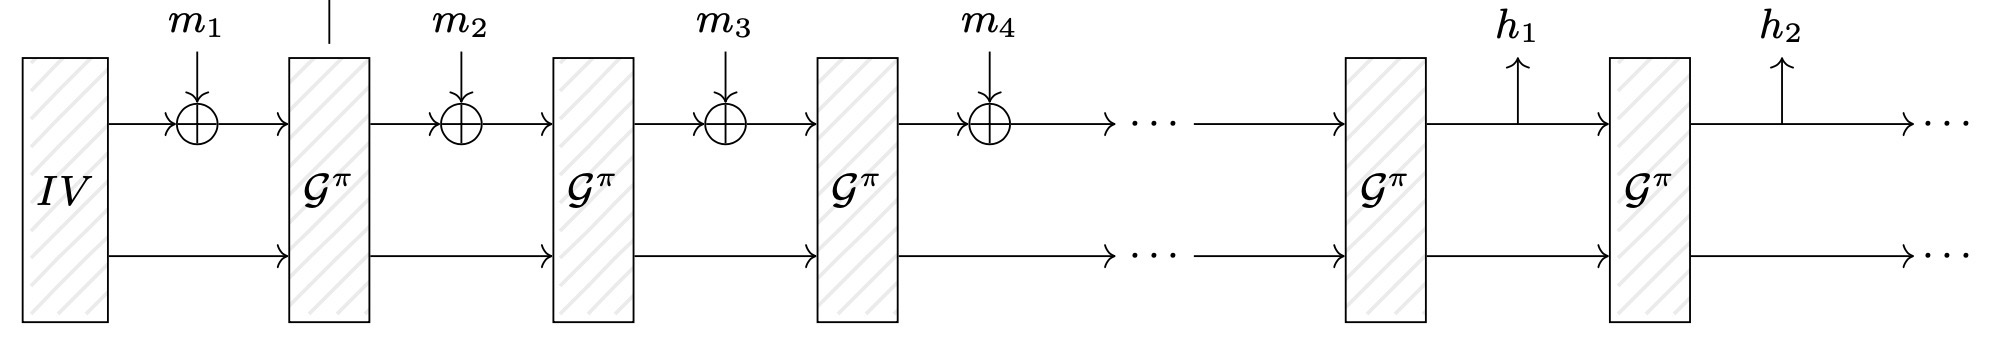
\includegraphics[width=\textwidth]{graphics/griffin-hash.png}
    \caption{Griffin-Sponge hash function~\cite{grassi2022horst}}
    \label{fig:griffin-hash}
\end{figure}

\begin{figure}[htbp]
    \centering
    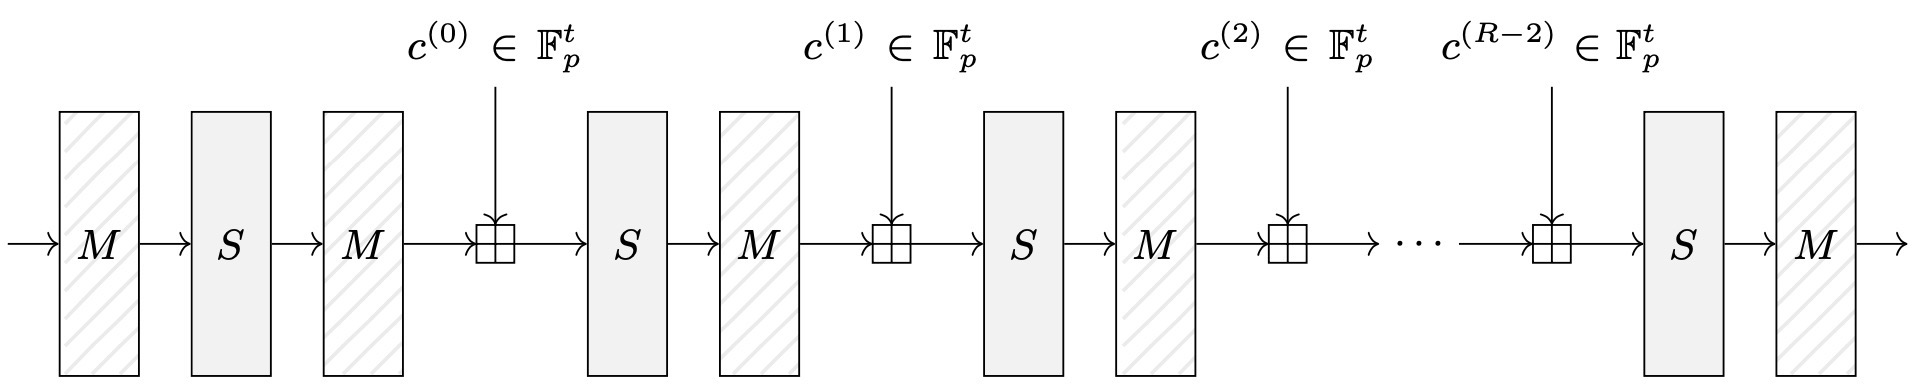
\includegraphics[width=\textwidth]{graphics/griffin-permutation.png}
    \caption{$\mathcal{G}^\pi$ permutation~\cite{grassi2022horst}}
    \label{fig:griffin-permutation}
\end{figure}

\section{Anemoi}
\label{sec:anemoi}
The Anemoi hash function~\cite{bouvier2023new} is also a very recent hash function, it was published by Bouvier et al. in 2023. It operates over a permutation, Anemoi$^\pi$, and this permutation works on a round function.\\
First we will start presenting the round function, next the permutation and finally the hash function.

\subsection*{Anemoi round function}
The Anemoi round function operates over the vector space $\mathbb{F}_q^{2l}$, where $l>0$, and $q$ is a prime number or a power of 2, in this thesis, we focus on $q=p$.

The length of the state is $2\times l$. In the Anemoi, the state is divided in two parts, the first part is $\left(x_0,\dots,x_{l-1}\right)$ and the second part is defined as $\left(y_0,\dots,y_{l-1}\right)$. We define a generator $g$ of the multiplicative subgrup of the field $\mathbb{F}_q$. If $q$ is prime, $g$ is the smallest generator, otherwiese $g$ is one of the roots of $\mathbb{F}_q = \mathbb{F}_{2^n}=\mathbb{F}_2[x]/p(x)$, where $p$ is an irreducible polynomial of degree $n$.

The structure of the Anemoi round function is composed of the following components: linear layer, S-box layer and constant addition. Figure~\ref{fig:anemoi-one-round} represents this structure.

Next, a description of each component is presented below.

\subsubsection*{Constant layer $\mathcal{A}$}
The constants layer corresponds to the addition of constants to the state vector, $x_j\leftarrow x_j+c_j^i$ and $y_j\leftarrow y_j+d_j^i$ where $c_j^i\in\mathbb{F}_q$ and $d_j^i\in\mathbb{F}_q$ are the round constants that depends on the position $i$ and the round $r$ of the permutation.\\
For calculating the round constants, we use
\begin{multline*}
    \pi_0=141592653589793238462643383279502884197169399375\\1058209749445923078164062862089986280348253421170679,
\end{multline*}
\begin{multline*}
    \pi_1=821480865132823066470938446095505822317253594081\\2848111745028410270193852110555964462294895493038196,
\end{multline*}
where $\pi_1$ and $\pi_2$ are the decimal expansion of $\pi$, and the computations for calculating the round constants $c_j^i$ and $d_j^i$ are
\begin{align}
    c_j^i=g\left(\pi_0^i\right)^2+\left(\pi_0^i+\pi_1^j\right)^\alpha \\
    d_j^i=g\left(\pi_1^j\right)^2+\left(\pi_0^i+\pi_1^j\right)^\alpha+g^{-1},
\end{align}

in the $\mathbb{F}_q$ field.

\subsubsection*{Linear layer $\mathcal{M}$}
In the Anemoi, the matrix M operates on the two vectors of the state $X=\left(x_0,\dots,x_{i-1}\right)$ and $Y=\left(y_0,\dots,y_{i-1}\right)$, separately. The matrix $M$ is defined as
\begin{equation}
    \mathcal{M}\left(X,Y\right)=\left(\mathcal{M}_x\left(X\right),\mathcal{M}_y\left(Y\right)\right),
\end{equation}
 $\mathcal{M}_x$ operates on the $X$ elements of the state and $\mathcal{M}_y$ on the $Y$ elements.\\
 We define $\mathcal{M}_x$ as a $l\times l$ matrix of $\mathbb{F}_q$ and $\mathcal{M}_y=\mathcal{M}_x\circ\rho$, where $\rho$ is a permutation over the $X$ vector defined as $\rho\left(x_0,\dots,x_{l-1}\right)=\left(x_1,\dots x_{l-1},x_0\right)$. The matrix $\mathcal{M}_x$ depends on the value of $l$. Depending on the $l$ size we separate two possible situations.
 \begin{itemize}
    \item $l$ is small, then the field size needs to be large.
    \item If $l$ is large, we expect a smallest field.
 \end{itemize}

 Similar to the previous hash functions, when $l \leq 4$ we can optimize the matrix and vector multiplications using the approach described in~\cite{duval2018mds}.\\
 In this cases, $l\in\{2,3,4\}$, the matrix $\mathcal{M}_x^l$ is
 \begin{equation}
    \mathcal{M}_x^2=
        \begin{pmatrix}
            1 & g \\
            g & g^2+1
        \end{pmatrix},\text{ }
    \mathcal{M}_x^3=
        \begin{pmatrix}
            g+1 & 1 & g+1 \\
            1 & 1 & g\\
            g & 1 & 1
        \end{pmatrix}, 
 \end{equation}
 \begin{equation}
    \mathcal{M}_x^4=
        \begin{pmatrix}
            1 & g^2 & g^2 & 1+g\\
            1+g & g+g^2 & g^2 & 1+2g \\
            g & 1+g & 1 & g \\
            g & 1+2g & 1+g & 1+g
        \end{pmatrix}.
 \end{equation}

 \subsubsection*{Pseudo-Hadamard transform $\mathcal{P}$}
 Anemoi uses a new layer that has not been used in the previous hash functions, it is used to increase the security after computing the S-box layer. It is very simple to implement, only needing two additions: $Y\leftarrow Y+X$ and $X\leftarrow X+Y$.
 
 \subsubsection*{Nonlinear layer $\mathcal{S}$}
 The nonlinear or S-box layer of the Anemoi also works different than in the previous hash functions. First we define the S-box as
 \begin{equation}
    \mathcal{S}\left(X,Y\right)=\left(\mathcal{H}\left(x_0,y_0\right),\dots,\mathcal{H}\left(x_{l-1,y_{l-1}}\right)\right),
 \end{equation}
where $\mathcal{H}$ is an \textit{open Flystel} (Section~\ref{sec:flyestel}) operating over $\mathbb{F}_q^2$. $\mathcal{H}$ uses 4 parameters, the exponent $\alpha$, the multiplier $\beta$, and the two constants $\gamma$ and $\delta$.\\
So, we let $\beta=g$, where $g$ has been defined before, $\delta\neq\gamma$, $\gamma=0$ and $\delta=g^{-1}$, and finally the exponent $\alpha$, that must satisfy gcd$\left(p-1,\alpha\right)=1$.

\begin{equation}
    \mathcal{H} = 
    \begin{cases}
        x_i\longleftarrow x_i-gQ(y_i)-g^{-1}\\
        y_i\longleftarrow y_i-x_i^{1/\alpha}\\
        x_i\longleftarrow x_i+Q(y_i)\\
    \end{cases}
\end{equation}

\begin{figure}[htbp]
    \centering
    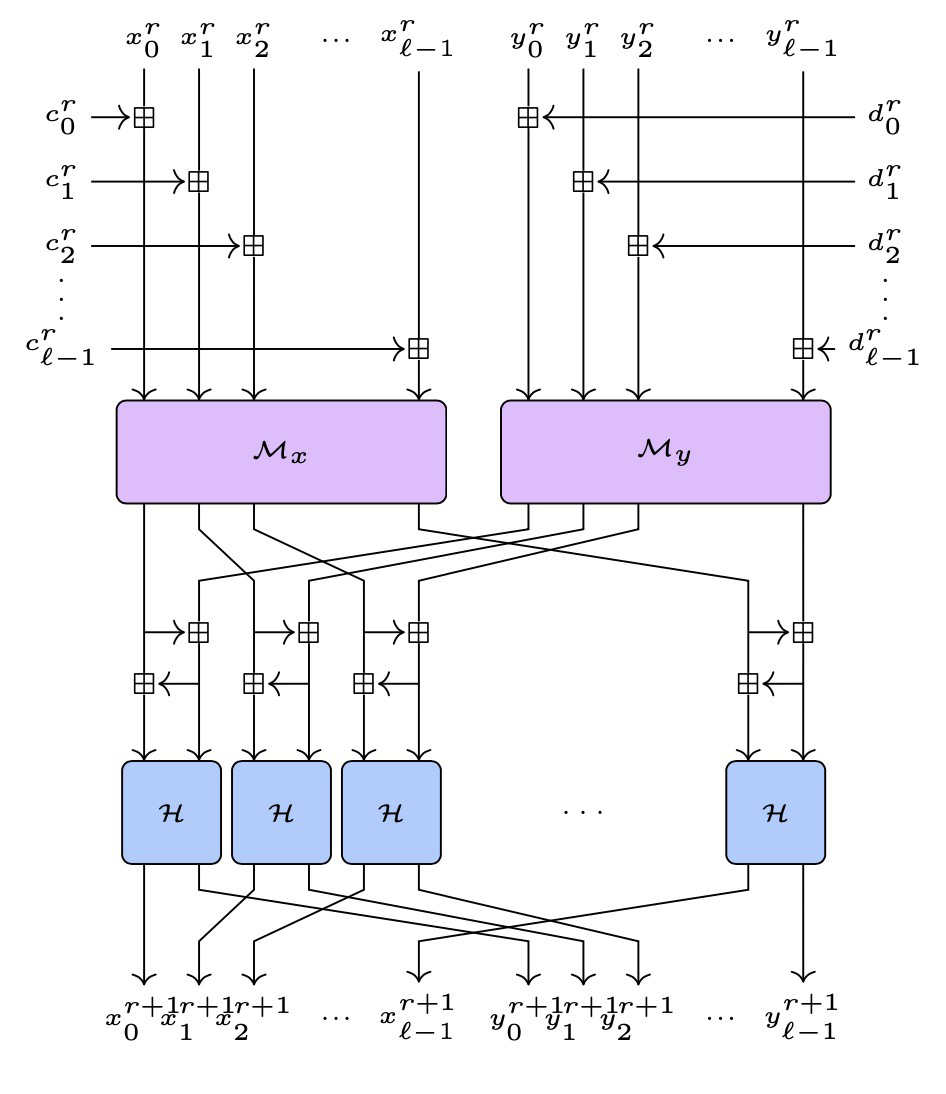
\includegraphics[width=0.8\textwidth]{graphics/anemoi-one-round.png}
    \caption{Round $r$ of Anemoi~\cite{bouvier2023new}}
    \label{fig:anemoi-one-round}
\end{figure}

\subsection*{Anemoi permutation}
The Anemoi permutation, Anemoi$^\pi$ iterates $n_r$ rounds over the round function previously explained, with a linear layer $\mathcal{M}$ when finishing the last round. It is defined as
\begin{equation}
    \text{Anemoi}^\pi_{q,\alpha,l}=\mathcal{M}\circ \text{R}_{n_r-1}\circ\dots \text{R}_0.
\end{equation}
where R$_i$ is the $i$ round function.\\
The number of rounds is computed using $\left(q,\alpha,l\right)$ with
\begin{equation}
    n_r\geq max\{
        8,\text{min}\left(5,1+l\right)+2+\text{min}\{r\in\mathbb{N}|\mathcal{C}_{alg(r)}\geq2^s\}\},
\end{equation}
where
\begin{equation}
    \begin{cases}
        \mathcal{C}_{alg(r)}=\left(\binom{4lr+k_\alpha}{2lr}^2\right) & \text{for } q=p, \\
        \mathcal{C}_{alg(r)}=lr\cdot9^{2lr} & \text{for } q=2^n
    \end{cases}
\end{equation}

\subsection*{Anemoi Hash}
The Anemoi hash function operates over the sponge construction in the field $\mathbb{F}_q^{r+c}$, as all the sponge constructions, $r$ values are used as the rate, and $c$ as the capacity.\\
We must take into consideration that the state has to be separated in $X$ and $Y$ with $l$ elements for each one, so the input must be even.

\subsubsection*{Sponge construction}
There is a modification of the mode of operation of the sponge construction explained in Section~\ref{sec:sponge-construction} and the one used in the Anemoi hash.\\
If we apply the standard sponge construction we may be applying the permutation, Anemoi$^\pi$, one more time when the length of the input is already a multiple of $r$. To solve this, we don't append more blocks at the end of the message if it is a multiple of $r$, rather, we add a constants $\sigma$ before the squeezing phase.\\
This constant $\sigma$ is equal to 0 if the message length is not multiple of $r$, and 1 if it is. Figure~\ref{fig:anemoi-sponge-mod} shows this modification, with $P$ being the Anemoi$^\pi$ permutation.
\begin{figure}[htbp]
    \centering
    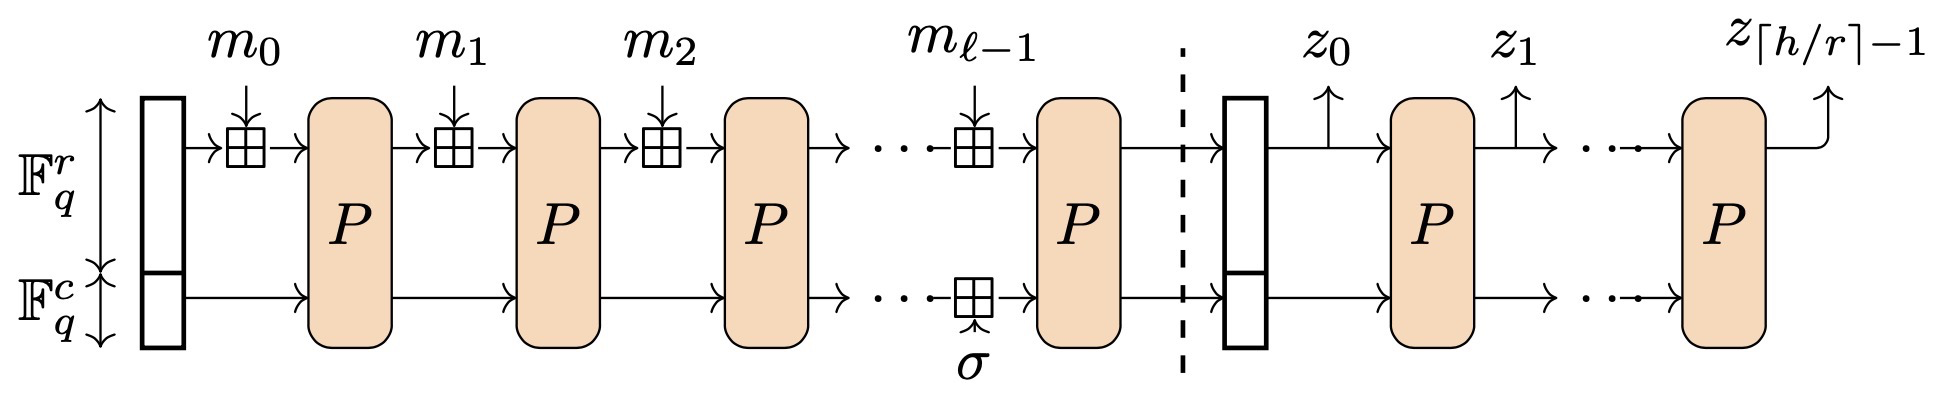
\includegraphics[width=\textwidth]{graphics/anemoi-sponge-mod.png}
    \caption{Anemoi-sponge~\cite{bouvier2023new}}
    \label{fig:anemoi-sponge-mod}
\end{figure}

\section{Arion}
\label{sec:Arion}
The Arion hash function~\cite{roy2023arion} was published by Roy et al. in 2023 and operates over a permutation, and on a lowest level there is the round function.\\
First we are going to explain the round function, followed by the permutation, and finally the hash function.

\subsection*{Arion round funtion}
The Arion hash function works on the $\mathbb{F}_p^t$ vector space, and is defined as
\begin{equation}
    \mathcal{R}_k^{(i)}(x)=\mathcal{K}_k\circ\mathcal{L}_{c_i}\circ\mathcal{F}_{Arion}^{(i)}(x)
\end{equation}

where $\mathcal{R}_k^{(i)}:\mathbb{F}_p^t\times\mathbb{F}_p^t$.

The structure of the Arion round function differs from the previous hash functions, it is composed of the following components: it starts with a GTDS, \textit{Generalized Triangular Dynamical System}~\cite{roy2022generalized}, followed by the affine layer and a keyed permutation.\\
Next, a description of each component is provided below.

\subsubsection*{GTDS Layer}
First, we define a field $\mathbb{F}_p$ with $p$ prime elements. Let $n,d_1,d_2,e\in\mathbb{Z}$ that
\begin{enumerate}
    \item $d_1$ is the smallest positive integer such that gcd$\left(d_1,p-1\right)=1$,
    \item $d_2$ is an integer such that gcd$\left(d_2,p-1\right)=1$,
    \item $e\cdot d_2\equiv1\text{ mod}\left(p-1\right)$. 
\end{enumerate}

The GTDS is defined as $\mathcal{F}_{Arion}=\{f_0,\dots,f_{t-1}\}$ for $1\leq i\leq t-1$, and $\alpha_{i,0},\alpha_{i,1},\beta_i\in\mathbb{F}_p$ so that $\alpha_{i,0}^2-4\cdot\alpha_{i,1}$ is a quadratic non-residue modulo $p$.\\
Thus,
\begin{equation}
    \begin{cases}
        f_i\left(x_0,\dots,x_{n-1}\right)=x_i^d\cdot g_i\left(\sigma_{i+1,t-1}\right)+h_i\left(\sigma_{i+1,t-1}\right), & 0\leq i\leq t-2, \\
        f_{t-1}\left(x_0,\dots,x_{t-1}\right)=x_{t-1}^e, & i=t-1,
    \end{cases}
\end{equation}
where
\begin{align}
    g_i(x)=x^2+\alpha_{i,0}\cdot x+\alpha_{i,1}, \\
    h_i(x)=x^2+\beta_i+x,
\end{align}
and
\begin{equation}
    \sigma_{i+1,t-1}=\sum_{j=i}^{t-1}x_j+f_j\left(x_0,\dots,x_{t-1}\right).
\end{equation}

\subsubsection*{Affine Layer}
The Affine Layer of Arion is defined over the vector space $\mathbb{F}_p^t$ as
\begin{equation}
    \mathcal{L}_c(x)=\text{circ}\left(0,\dots,t-1\right)x+c,
\end{equation}
where circ$\left(0,\dots,t-1\right)$ is the circulant matrix with the first row being $\left(1,\dots,t-1\right)$ and $c\in\mathbb{F}_p^t$ is the constant vector.

\subsubsection*{Keyed permutation}
The keyed permutation, $\mathcal{K}_k$, works over the field $\mathbb{F}_p^t$. It is defined as
\begin{equation}
    \mathcal{K}_k\left(x,k\right)=x+k.
\end{equation}

\subsection*{Arion permutation}
The Arion permutation: $\mathbb{F}_p^t\times\mathbb{F}_p^t\times\left(r+1\right)\rightarrow\mathbb{F}_p^t$ is defined as
\begin{equation}
    \text{Arion}^\pi(x,k_0,\dots,k_{r-1})=\mathcal{R}_{k_{r-1}}^{(r-1)}\circ\dots\circ\mathcal{R}_{k_0}^{(0)}\circ\mathcal{L}_0\circ\mathcal{K}_{k_0}(x)
\end{equation}
for $0\leq i\leq r-1$, where $r$ is the number of rounds of the permutation.\\
Furthermore, the Arion$^\pi$ is instantiated with the key $k_0=\dots=k_{r-1}=0$.

\subsection*{Arion hash}
The Arion hash function works in the field $\mathbb{F}_p^t$ and over the sponge construction. As a sponge construction, the length of the state is $t=r+c$, where $r$ is the rate and $c$ the capacity.

\chapter{Implementation}
\label{sec:impl}
We have developed two libraries to evaluate the performance of the hash functions discussed in Section~\ref{sec:zk-hashes}. The first library uses the Plonky2\footnote{\url{https://github.com/0xPolygonZero/plonky2}} proving system from Polygon Labs, a SNARK proving system based on PLONK and FRI, allowing us to write these functions as arithmetic circuits and generate proofs of knowledge.\\
The second library implements these functions using Dusk Plonk\footnote{\url{https://github.com/dusk-network/plonk}} from Dusk Network, a Plonk proving system as descrived in section~\ref{sec:plonk}.

In addition to zero-knowledge implementations, we also incorporated the plain implementation of such hash functions.

Both libraries are written in the Rust programming language and designed to allow future inclusions of additional hash functions.

Rust was chosen as the programming language due to its compatibility with both Plonky2 and PLONK, given that these frameworks are implemented in Rust.

Both libraries are not stable, meaning that they are under active development, so for using them we can't use the Stable Rust version, we worked on the Nightly version.

These hash functions are constructed based on the concepts provided in section~\ref{sec:zk-hashes}. Note that, we used SageMath to compute the constants of the hashes and create binary files to store them. SageMath was selected for his ability in algebra over finit fields and the broader range of mathematical functionalities it provides.

Additionally, we used Criterion, a benchmarking library in Rust, to check the performance of the hashes in both libraries, in the standard and zero-knowledge.

\section{Implementation using Plonky2}
\label{sec:plonky-implementation}
Plonky2 operates on the Goldilocks field (section~\ref{sec:goldilocks}), $p=2^{64} - 2^{32} + 1$. We used SageMath for the generation of round constants, MDS matrices, and number of rounds for each hash function.

The implementation is divided into four parts:
\begin{enumerate}
  \item \textbf{Circuit setup}. Firts, we generate the virtual targets\footnote{The term virtual target refers to an intermediate value used during the setup of the circuit but not used in the computation during proof generation.}, such as the private input and the state of the sponge. Subsequently, we check that the input $\geq0$ and is multiple of the rate $r$. Next, we develop the arithmetic circuit, in our case, it corresponds to the algorithm of each hash function, including the absorbing and the digest part, to generate the output based on the chosen length, and finally assing it as the public input.
  \item \textbf{Witness generation}. Here, we assing the values of the private inputs (witnesses), such as the inputs and the constants of the hash function.
  \item \textbf{Proof generation}. Internally, in the Plonky2 framework, the circuit is constructed, all the constraints of the circuit are generated, including copy constraints, forming the constraint system. Afterwards, the witnesses are used to evaluate the constraint system, generating the proof following the procedure explained in section~\ref{sec:plonk}.
  \item \textbf{Proof verification}. Finally, the circuit is verified, the verifier using the proof alognside the public inputs decides if he accepts the proof or not.
\end{enumerate}

We only conducted tests for a state length $t=12$, contrary to the Plonk implementation. Plonky2 is an upgraded version of Plonk, and there are some automatic optimizations to reduce the number of constraints, thus, improving efficiency. Table~\ref{tab:goldi-rounds} shows the round numbers for the hashes that we implement in the Goldilocks field, where $\alpha$ is the smallest integer value for wich $x^\alpha$ is a permutation, in other words, $gcd(p-1,\alpha)=1$.

\begin{table}[htbp]
  \centering
  \begin{tabular}{@{}cccccc@{}}
  \toprule
  \multicolumn{6}{c}{Rounds}                                           \\ \midrule
  \multicolumn{1}{c|}{Hash} &
    \multicolumn{1}{c|}{Poseidon} &
    \multicolumn{1}{c|}{Rescue-prime} &
    \multicolumn{1}{c|}{Griffin} &
    \multicolumn{1}{c|}{Anemoi} &
    \multicolumn{1}{c|}{Arion} \\ \midrule
  \multicolumn{1}{l|}{State size $t$} & \multicolumn{5}{c}{$\alpha=7$} \\ \midrule
  \multicolumn{1}{c|}{12} &
    \multicolumn{1}{c|}{$r_f=8,$ $r_p=22$} &
    \multicolumn{1}{c|}{7} &
    \multicolumn{1}{c|}{8} &
    \multicolumn{1}{c|}{10} &
    \multicolumn{1}{c|}{4} \\ \bottomrule
  \end{tabular}
  \caption{Round numbers for Poseidon [Section~\ref{sec:poseidon}], Rescue-prime [Section~\ref{sec:Rescue-prime}], Griffin [Section~\ref{sec:griffin}], Anemoi [Section~\ref{sec:anemoi}], Arion [Section~\ref{sec:Arion}]}
  \label{tab:goldi-rounds}
  \end{table}

\textbf{Optimizations}\\
The main goal of this optimization is to improve the efficiency of the circuit by reducing the computational complexity and the number of constraints.\\
We optimized certain computations of the code to minimize the number of constraints. The inverse S-box involves the calculation of $x^{1/d}$. Instead of computing $x^{1/d}$ directly, we first compute $y^d$ within the circuit, where $y$ is a new virtual target representing the inverse operation. This allows us to simplify the exponentiation to a series of multiplications, which are computationally cheaper.\\
Subsequently, we compute $x$ from $y^d$ during circuit design rather than during proof generation phase. Finally, we connect $x$ and $y^d$. This is done by establishing a constraint within the circuit that binds the outcome of $y^d$ to the original value $x$.

In the following code, we implement this optimization.

First of all, we define a trait that implements CircuitBuilder, used to build constraints, add witnesses, generally, to setup the circuit, and we define a function used to compute $x^{1/d}$. Next, we create a virtual target $y$ and with it we compute $y^d$. Subsequently, we add a generator, it assigns a value to a virtual target during proof generation. In this generator we compute the expensive operation $x^{1/d}$, this operation is computed once during circuit setup and not during proof generation.

Finally we ensure that the result from the operation $x^{1/d}$ is correctly linked to the previously established virtual target $y$, so $y=x^{1/d}$.
\vspace{1em}

\begin{lstlisting}
trait CircuitBuilderExtensions<F: RichField + Extendable<D>, const D: usize> {
    fn exp_inv(&mut self, x: Target) -> Target;
    fn exp_inv_extension(&mut self, x: ExtensionTarget<D>) -> ExtensionTarget<D>;
}

impl<F: RichField + Extendable<D>, const D: usize> CircuitBuilderExtensions<F, D> 
  for CircuitBuilder<F, D>
{
  fn exp_inv(&mut self, x: Target) -> Target {
      let x_ext = self.convert_to_ext(x);
      Self::exp_inv_extension(self, x_ext).0[0]
  }

  fn exp_inv_extension(&mut self, x: ExtensionTarget<D>) -> ExtensionTarget<D> {
      let exp_inv = self.add_virtual_extension_target();
      self.add_simple_generator(ExpGeneratorExtension {
          base: x,
          exp_result: exp_inv,
      });

      // Enforce that y^d = x
      // d = 7 (ALPHA)
      let x2 = self.mul_extension(exp_inv, exp_inv);
      let x4 = self.mul_extension(x2, x2);
      let x6 = self.mul_extension(x4, x2);
      let y_inv = self.mul_extension(x6, exp_inv);
      self.connect_extension(y_inv, x);

      exp_inv
  }
}

#[derive(Debug, Default)]
pub struct ExpGeneratorExtension<const D: usize> {
    base: ExtensionTarget<D>,
    exp_result: ExtensionTarget<D>,
}

impl<F: RichField + Extendable<D>, const D: usize> SimpleGenerator<F, D>
    for ExpGeneratorExtension<D>
{
    fn id(&self) -> String {
        "ExpGeneratorExtension".to_string()
    }

    fn dependencies(&self) -> Vec<Target> {
        let deps = self.base.to_target_array().to_vec();
        deps
    }

    fn run_once(
        &self,
        witness: &plonky2::iop::witness::PartitionWitness<F>,
        out_buffer: &mut plonky2::iop::generator::GeneratedValues<F>,
    ) {
        let base = witness.get_extension_target(self.base);
        let mut current_base = base.clone();
        let mut exp = <F as Extendable<D>>::Extension::from(F::ONE);
        let mut power = ALPHA_INV;
        while power > 0 {
            if power % 2 == 1 {
                exp = exp * current_base;
            }
            current_base = current_base * current_base;
            power /= 2;
        }
        out_buffer.set_extension_target(self.exp_result, exp)
    }

    fn serialize(
        &self,
        dst: &mut Vec<u8>,
        _common_data: &plonky2::plonk::circuit_data::CommonCircuitData<F, D>,
    ) -> plonky2::util::serialization::IoResult<()> {
        dst.write_target_ext(self.base)?;
        dst.write_target_ext(self.exp_result)
    }

    fn deserialize(
        src: &mut plonky2::util::serialization::Buffer,
        _common_data: &plonky2::plonk::circuit_data::CommonCircuitData<F, D>,
    ) -> plonky2::util::serialization::IoResult<Self> {
        let base = src.read_target_ext()?;
        let exp = src.read_target_ext()?;
        core::result::Result::Ok(Self {
            base,
            exp_result: exp,
        })
    }
}
\end{lstlisting}


\section{Implementation using Dusk Plonk}
In the Plonk implementation of the Dusk Network, we operate on the BLS12-381 curve, detailed in section~\ref{sec:bls12}, using $r$ as the modulus of the field.

\textbf{Plonk modifications.} In this Plonk framework, there is a modification in the two input Plonk constraint detailed in Equation~\ref{eq:plonk-constraint}. However, in this framework, the Plonk equation has 3 inputs (3 addition gates)
\begin{equation}
  \left(\textbf{q}_\textbf{L}\right)_i\cdot\textbf{x}_{\textbf{a}_i}+ \left(\textbf{q}_\textbf{R}\right)_i\cdot\textbf{x}_{\textbf{b}_i} + \left(\textbf{q}_\textbf{O}\right)_i\cdot\textbf{x}_{\textbf{ac}_i} + \left(\textbf{q}_\textbf{M}\right)_i\cdot\left(\textbf{x}_{\textbf{a}_i}\textbf{x}_{\textbf{b}_i}\right) + \left(\textbf{q}_\textbf{C}\right)_i + \left(\textbf{q}_\textbf{F}\right)_i\cdot\textbf{x}_{\textbf{d}_i}=0
\end{equation}

where $d$ is the "fourth" variable and $\textbf{q}_\textbf{F}$ the selector coefficient.

We integrated the hash functions directly to the Dusk Network repository\footnote{\url{https://github.com/dusk-network/Poseidon252}}, with the exception of the Poseidon hash function, which was already available. To acommodate the hash functions from Section~\ref{sec:zk-hashes}, we generalized the code.

The implementation is the same as in the Plonky2, due to Plonky2 being based on the PLONK proving system.

For the generation of round constants and MDS matrices, we again used SageMath. However, due to the significant size of the field, reaching up to 256 bits, we can't store the values directly. Therefore, after obtaining the values using SageMath, we converted them into an array of 32 bytes, configuring the byte order to be "little-endian" to ensure the most significant byte is at the end of the byte array. After that, we create a binary file to store the these computed constants. For using them on the code, they were then mapped onto "BlsScalar" in the BLS12-381 scalar field.

In the Plonk implementation we conducted tests for $t\in{4,5,6,8}$. Table~\ref{tab:plonk-rounds} shows the round numbers for each hash function and their state length $t$.

\begin{table}[htbp]
  \centering
  \begin{tabular}{@{}cccccclll@{}}
  \toprule
  \multicolumn{9}{c}{Rounds}                                                                                                                                              \\ \midrule
  \multicolumn{1}{l|}{} &
    \multicolumn{1}{c|}{Poseidon} &
    \multicolumn{1}{c|}{Rescue-prime} &
    \multicolumn{1}{c|}{Griffin} &
    \multicolumn{1}{c|}{Anemoi} &
    \multicolumn{4}{c}{Arion} \\ \midrule
  \multicolumn{1}{l|}{$t$} & \multicolumn{8}{c}{$\alpha=5$}                                                                                                               \\ \midrule
  \multicolumn{1}{c|}{4}   & \multicolumn{1}{c|}{$r_f=8,$ $r_p=56$} & \multicolumn{1}{c|}{11} & \multicolumn{1}{c|}{11} & \multicolumn{1}{c|}{12} & \multicolumn{4}{c}{5} \\
  \multicolumn{1}{c|}{5}   & \multicolumn{1}{c|}{$r_f=8,$ $r_p=60$} & \multicolumn{1}{c|}{9}  & \multicolumn{1}{c|}{-}  & \multicolumn{1}{c|}{-}  & \multicolumn{4}{c}{5} \\
  \multicolumn{1}{c|}{6}   & \multicolumn{1}{c|}{$r_f=8,$ $r_p=57$} & \multicolumn{1}{c|}{8}  & \multicolumn{1}{c|}{-}  & \multicolumn{1}{c|}{10} & \multicolumn{4}{c}{5} \\
  \multicolumn{1}{c|}{8}   & \multicolumn{1}{c|}{$r_f=8,$ $r_p=57$} & \multicolumn{1}{c|}{8}  & \multicolumn{1}{c|}{9}  & \multicolumn{1}{c|}{10} & \multicolumn{4}{c}{4} \\ \bottomrule
  \end{tabular}
  \caption{Round numbers for Poseidon [Section~\ref{sec:poseidon}], Rescue-prime [Section~\ref{sec:Rescue-prime}], Griffin [Section~\ref{sec:griffin}], Anemoi [Section~\ref{sec:anemoi}], Arion [Section~\ref{sec:Arion}]}
  \label{tab:plonk-rounds}
  \end{table}

Note that, the length of the state in Griffin must be 3 or a multiple of 4 as explained in section~\ref{sec:griffin} and in Anemoi it must be even, outlined in section~\ref{sec:anemoi}.

To improve efficiency, we perform the same optimization used in Plonky2 to reduce number of constraints in the Plonk framework.

In the following code, the optimization over the Plonk framework is conducted.\\
We can see that the approach to compute $x^{1/d}$ is more simplier than in the Plonky2 framework. However, both of these implementation follow the same idea to optimize this operation.

In Plonk, the Composer is the same as the CircuiBuilder in Plonky2, it handles the arrangement and management of computations and constraints within the circuit.

We start by retrieving the value assigned to a witness variable $x$ which is used to compute $x^{1/d}$. Once the operation on $x$ is computed, this value is allocated within the composer, and its index is stored. This index represents $y$, and is used to compute $y^{1/d}$. The final step involves ensuring that the original witness $x$ is consistent with the computed index from $y^{1/d}$. This is necesary for ensuring that they conform to the circuit constraints.
\vspace{1em}

\begin{lstlisting}
  fn inverse_sbox(&mut self, value: &mut Witness) {
      // Retrieve the value from the composer and compute a power operation
      let tmp = self.composer[*value];
      let tmp = tmp.pow_vartime(&E_2);

      // Allocate the computed value as a new witness in the composer
      let wit = self.composer.append_witness(tmp);

      // y^2
      let constraint = Constraint::new().mult(1).a(wit).b(wit);
      let tmp_wit = self.composer.gate_mul(constraint);
      // y^4
      let constraint = Constraint::new().mult(1).a(tmp_wit).b(tmp_wit);
      let tmp_wit = self.composer.gate_mul(constraint);
      // Compute y^5 by multiplying y^4 with y, and update the original witness value
      let constraint = Constraint::new().mult(1).a(tmp_wit).b(wit);
      *value = self.composer.gate_mul(constraint);
      *value = wit;
    }
\end{lstlisting}

\chapter{Evaluation}
\label{sec:evaluation}
\section*{Overview}
In this section, we provide a comparative analysis of the implemented hash functions from section~\ref{sec:zk-hashes}, including Poseidon, Rescue-prime, Griffin, Anemoi and Arion on the Plonky2 and Plonk proving sytems.

Our objective with these measurement is to provide a realistic perspective and reason about the user decision when using these hash functions.

\section{Specifications}
Measurements were conducted on a system configured with a 1.4 GHz Quad-Core Intel Core i5 processor, 8 GB LPDDR3 RAM with a transfer rate of 2133 MHz, and running macOS 14.5. The system was clocked at 1.4 GHz and utilized Rust's Nightly build dated 2024-02-01. Benchmarking was performed using Criterion 0.5, with Plonky2 version 0.1.4 and dusk-plonk version 0.19.

\section{Plonky2 Performance}

In Table~\ref{tab:goldi-plain-performance}, the plain performance on the Goldilocks field is compared using the number of rounds specified in Table~\ref{tab:goldi-rounds}.

From this metrics, we can observe that Arion and Griffin shows the best performance with the shortest execution time compared to Rescue and and Anemoi. However, as we show later in Table~\ref{tab:plonky2-performance}, Arion has a worst performance when used in SNARKs over the Goldilocks field. Rescue and Anemoi have the worst plain performance due to having many $x^{1/\alpha}$ evaluations per round. Griffin and Arion also uses $x^{1/\alpha}$, but only once per round. Poseidon, despite having a high number of rounds, doesn't compute inverse S-box so its performance is as good as Arion and Griffin.

\begin{table}[htbp]
  \centering
  \begin{tabular}{@{}cclllc@{}}
  \toprule
  \multicolumn{6}{c}{Time (µs)}                                \\ \midrule
  \multicolumn{1}{l|}{}               & \multicolumn{5}{c}{Hash}       \\ \cmidrule(l){2-6} 
  \multicolumn{1}{l|}{}   & \multicolumn{1}{l}{Poseidon} & Rescue-prime                  & Griffin                       & Anemoi                        & Arion     \\ \midrule
  \multicolumn{1}{c|}{State size $t$} & \multicolumn{5}{c}{$\alpha=7$} \\ \midrule
  \multicolumn{1}{c|}{12} & 8.1879                    & \multicolumn{1}{c}{23.293} & \multicolumn{1}{c}{4.6652} & \multicolumn{1}{c}{32.266} & 3.6192 \\ \bottomrule
  \end{tabular}
  \caption{Plain performance comparasion on the Goldilocks field.}
  \label{tab:goldi-plain-performance}
  \end{table}

Table~\ref{tab:plonky2-performance} presents metrics for circuit setup and proof generation of all hash functions in the Plonky2 framework within the Goldilocks field.\\
Circuit setup and proof generation times reflect the complexity and computational demands of integrating the hash functions into the zero-knowledge framework.

In this table we can see that, Anemoi, Griffin and Arion show the most efficient circuit setup times around 33 ms, meaning that their circuit design are less complex than in the case of Poseidon and Rescue, for the same reasons we explained before.\\
Anemoi presents better metrics than in plain performance, due to being able to apply the optimization to compute $x^{1/\alpha}$ as it is explained in section~\ref{sec:plonky-implementation}.\\
Poseidon has the longest proof generation time (114,32 ms), which indicate a higher number of constraint in the circuit design, due to the high round number it has. Arion, we can see that it has a moderately high proof generation time, indicating that it is not optimized to work on the Goldilocks field, in contrast, in Table~\ref{tab:plonk-performance} it presentes good results when working on the BLS12-381 curve.

\begin{table}[htbp]
  \centering
  \resizebox{\textwidth}{!}{%
  \begin{tabular}{@{}cccccccllll@{}}
  \toprule
  \multicolumn{11}{c}{Time (ms)}                                                                                  \\ \midrule
  \multicolumn{1}{c|}{}               & \multicolumn{5}{c|}{Circuit Setup} & \multicolumn{5}{c}{Proof Generation} \\ \midrule
  \multicolumn{1}{c|}{Hash} &
    Poseidon &
    Rescue-prime &
    Griffin &
    Anemoi &
    \multicolumn{1}{c|}{Arion} &
    \multicolumn{1}{l}{Poseidon} &
    Rescue-prime &
    Griffin &
    Anemoi &
    Arion \\ \midrule
  \multicolumn{1}{l|}{State size $t$} & \multicolumn{10}{c}{$\alpha=7$}                                           \\ \midrule
  \multicolumn{1}{c|}{12} &
    79,575 &
    42.081 &
    33.891 &
    33.778 &
    \multicolumn{1}{c|}{33,806} &
    114.32 &
    \multicolumn{1}{c}{74.845} &
    \multicolumn{1}{c}{75.450} &
    \multicolumn{1}{c}{74.802} &
    \multicolumn{1}{c}{89,75} \\ \bottomrule
  \end{tabular}%
  }
  \caption{Plonky2 performance comparasion.}
  \label{tab:plonky2-performance}
  \end{table}


\section{Plonk Performance}

In Table~\ref{tab:bls-plain-performance}, we evaluate the plain implementation of the hash functions within the BLS12-381 curve using the round numbers from Table~\ref{tab:plonk-rounds}.

As the table shows, Poseidon and Arion are the fastest permutations, reinforcing the results obtained in Table~\ref{tab:goldi-plain-performance}. Similar to previous observations, Rescue and Anemoi have the lowest performance, fundamentally due to the number of $x^{1/\alpha}$ operations required to compute in one round. In contrast, Griffin maintains comparable results for different state size $t$.

As we can see, for smaller state size $t$ the performance is better than for a larger $t$, due to the cost of high computational operations needed to be evaluated per round. If we take a look at Table~\ref{tab:plonk-rounds}, we can observe that we have more rounds for smallest $t$ and less for larger $t$, with this, we may believe that we will have better performance for bigger $t$, but looking at the results we can conclude that the state size is more influential than the number of rounds.

\begin{table}[htbp]
  \centering
  \begin{tabular}{@{}cccccc@{}}
  \toprule
  \multicolumn{6}{c}{Time (µs)}                                \\ \midrule
  \multicolumn{1}{l|}{}               & \multicolumn{5}{c}{Hash}       \\ \cmidrule(l){2-6} 
  \multicolumn{1}{l|}{}  & \multicolumn{1}{l}{Poseidon}   & \multicolumn{1}{l}{Rescue-prime} & \multicolumn{1}{l}{Griffin}    & \multicolumn{1}{l}{Anemoi}     & Arion     \\ \midrule
  \multicolumn{1}{c|}{State size $t$} & \multicolumn{5}{c}{$\alpha=5$} \\ \midrule
  \multicolumn{1}{c|}{4} & \multicolumn{1}{c|}{47,89}  & \multicolumn{1}{c|}{776,98}   & \multicolumn{1}{c|}{206,96} & \multicolumn{1}{c|}{421,56} & 94,76  \\
  \multicolumn{1}{c|}{5} & \multicolumn{1}{c|}{73,308} & \multicolumn{1}{c|}{795,47}   & \multicolumn{1}{c|}{-}         & \multicolumn{1}{c|}{-}         & 96,84  \\
  \multicolumn{1}{c|}{6} & \multicolumn{1}{c|}{99,2}   & \multicolumn{1}{c|}{856,76}   & \multicolumn{1}{c|}{-}         & \multicolumn{1}{c|}{525,08} & 100,25 \\
  \multicolumn{1}{c|}{8} & \multicolumn{1}{c|}{166,06} & \multicolumn{1}{c|}{1146}    & \multicolumn{1}{c|}{221,51} & \multicolumn{1}{c|}{704,67} & 84,649 \\ \bottomrule
  \end{tabular}
  \caption{Plain performance comparison on the BLS12-381 scalar field.}
  \label{tab:bls-plain-performance}
  \end{table}

Next, we will provide metrics for the hash functions implemented in the Plonk framework within the BLS12-381 curve.

Table~\ref{tab:plonk-constraints} compare the efficiency of the different hash functions in Plonk by counting the number of constraints required to compute the proof.\\
The table indicates that as the state size $t$ increases, the number of constraints typically increases as well for all hash functions. This trend suggests that larger state sizes require more computational resources, which align with the expected increase in the complexity of the computation.

Arion is the most efficient in terms of constraints requirements across all tested state sizes. Making it suitable for systems where performance is important.\\
Poseidon starts at a resonable constraint count for smaller states, esclates faster than the other hashes due to his high number of rounds.\\
Anemoi and Griffin demonstrate a consistent increase of constraints when increasing the state size.


\begin{table}[htbp]
  \centering
  \begin{tabular}{@{}lccccclll@{}}
  \toprule
  \multicolumn{9}{c}{Plonk Constraints} \\ \midrule
  \multicolumn{1}{c|}{} &
    \multicolumn{8}{c}{Hash} \\ \cmidrule(l){2-9} 
  \multicolumn{1}{l|}{} &
    \multicolumn{1}{l}{Poseidon} &
    \multicolumn{1}{l}{Rescue-prime} &
    \multicolumn{1}{l}{Griffin} &
    \multicolumn{1}{l}{Anemoi} &
    \multicolumn{4}{l}{Arion} \\ \midrule
  \multicolumn{1}{l|}{State size $t$} &
    \multicolumn{8}{c}{$\alpha=5$} \\ \midrule
  \multicolumn{1}{l|}{4} &
    \multicolumn{1}{c|}{788} &
    \multicolumn{1}{c|}{536} &
    \multicolumn{1}{c|}{356} &
    \multicolumn{1}{c|}{328} &
    \multicolumn{4}{c}{241} \\
  \multicolumn{1}{l|}{5} &
    \multicolumn{1}{c|}{995} &
    \multicolumn{1}{c|}{550} &
    \multicolumn{1}{c|}{-} &
    \multicolumn{1}{c|}{-} &
    \multicolumn{4}{c}{305} \\
  \multicolumn{1}{l|}{6} &
    \multicolumn{1}{c|}{1501} &
    \multicolumn{1}{c|}{682} &
    \multicolumn{1}{c|}{-} &
    \multicolumn{1}{c|}{412} &
    \multicolumn{4}{c}{367} \\
  \multicolumn{1}{l|}{8} &
    \multicolumn{1}{c|}{2461} &
    \multicolumn{1}{c|}{1034} &
    \multicolumn{1}{c|}{866} &
    \multicolumn{1}{c|}{634} &
    \multicolumn{4}{c}{406} \\ \bottomrule
  \end{tabular}
  \caption{Plonk constraint comparasion. Round numbers are the same as in Table~\ref{tab:plonk-rounds}}
  \label{tab:plonk-constraints}
  \end{table}


The Table~\ref{tab:plonk-performance} shows performance metrics for the circuit setup and proof generation times of the hash functions implemented using Plonk in the BLS12-381 curve.

In the circuit setup, the times generally increase with the state size for most hash functions.

Poseidon and Rescue-prime show very similar setup times for smaller state sizes but when $t\geq6$ Poseidon shows an increase and Anemoi also for $t=8$.

Arion stands out as the most efficient and scalable in both circuit setup and proof generation. In contrast to the implementation in Plonky2 over the Goldilocks field, in the Plonk framework over the BLS12-381, it presents the best performance over all the hashes making it more suitable when working over the BLS12-381 curve than in the Goldilocks field.\\
Poseidon, similar to the previous tables, shows increases in both circuit setup and proof generation times as state size increase.\\
Griffin, Anemoi and Arion, the three of them perform the inverse S-box only one time per round, as previously explained, but Arion having less number of rounds than the previous hashes makes it more efficient in circuit setup and proof generations.

\begin{table}[htbp]
  \resizebox{\textwidth}{!}{%
  \begin{tabular}{@{}lllllllll@{}}
  \toprule
  \multicolumn{9}{c}{Time (ms)}                                                                                                                                                       \\ \midrule
  \multicolumn{1}{c|}{}             & \multicolumn{4}{c|}{Circuit setup}                                                         & \multicolumn{4}{c}{Proof generation}                       \\ \cmidrule(l){2-9} 
  \multicolumn{1}{c|}{}             & \multicolumn{8}{c}{State size $t$}                                                                                                                      \\ \midrule
  \multicolumn{1}{l|}{}             & 4         & 5                     & 6                     & \multicolumn{1}{l|}{8}         & 4          & 5         & 6                     & 8         \\ \midrule
  \multicolumn{1}{l|}{Hash}         & \multicolumn{8}{c}{$\alpha=5$}                                                                                                                          \\ \midrule
  \multicolumn{1}{l|}{Poseidon}     & 814,58 & 811,16             & 1514,4              & \multicolumn{1}{l|}{2489,1} & 766,25  & 761,49 & 1465,1             & 2337,9  \\
  \multicolumn{1}{l|}{Rescue-prime} & 812,88 & 812,62             & 813,4              & \multicolumn{1}{l|}{1507,6}    & 770,11  & 766,81 & 773,95             & 1421,8  \\
  \multicolumn{1}{l|}{Griffin}      & 434,83 & \multicolumn{1}{c}{-} & \multicolumn{1}{c}{-} & \multicolumn{1}{l|}{809,59} & 437,83  & -         & \multicolumn{1}{c}{-} & 835,42 \\
  \multicolumn{1}{l|}{Anemoi}       & 435,18 & \multicolumn{1}{c}{-} & 437,03             & \multicolumn{1}{l|}{812,83} & 422, 63 & -         & 414,32             & 784,38 \\
  \multicolumn{1}{l|}{Arion}        & 303,07 & 436,53             & 436,76             & \multicolumn{1}{l|}{437,69} & 293,58  & 412,53 & 418,73             & 417,21 \\ \bottomrule
  \end{tabular}%
  }
  \caption{Plonk performance comparasion. Round numbers are the same as in Table~\ref{tab:plonk-rounds}}
  \label{tab:plonk-performance}
  \end{table}

\chapter{Conclusions}
\label{sec:conclusions}
\section{Discussion}
This thesis succesfully developed and evaluated a series of hash functions within two zero-knowledge frameworks, namely Plonky2 and Plonk, focusing on the generation of proofs of knowledge for these computed hashes.

In chapter~\ref{sec:theory}, we provide the theoretical knowledge needed to understand the development of the project. This include some background knowledge on hash functions, sponge structure and finit fields, forming a solid foundation for understanding zero-knowledge proofs and the specific proving system we are using in this thesis, Plonk.

Chapter~\ref{sec:impl} discusses the implementation of these hash functions, highlighting significant optimizations that improve performance, particulary within the zero-knowledge framework. Benchmarking results indicate that the implemented hash functions meet the expected performance regarding their characteristics, as explained in section~\ref{sec:zk-hashes}.

So, which is the best hash function? As is often the case, the answer is not that simple and depends of various factors, such as the chosen zero-knowledge proof system and the primary cost metric for the use case. Let's first investigate the best hash function considering prover performance, in other words, minimizing the number of constraints inside the cicuit. Since Poseidon, the objective has been to minimize the number of multiplications within the circuit. This led to using both $y=x^d$ and $y=x^{1/d}$, which results in a secure hash function with a small number of rounds (and thus also a small number of constraints). The first hash functions to implement this is Rescue, followed by new optimizations that let to the development of Griffin, Anemoi and Arion. We compared these hash functions for performance when used in various configurarions and proof systems. From the results obtained in Chapter~\ref{sec:evaluation}, Arion shows better performance when used in Plonk proof system compared to all other hash functions. In contrast, in the Plonky2 proving system, Rescue, Griffin and Anemoi, each with similar performance, perform better than Arion.

What makes these hash functions, Griffin, Rescue, Anemoi and Arion so fast inside the zero-knowledge circuit makes them slow for plain hashing. Consequently, for cases where plain performance is equally important as the prover performance, the hash function with best performance differs from the previous results. Here, we need to consider the prime field we are working on. In this thesis, we implemented them in two field, the Goldilocks and the BLS12-381 scalar field. In the case of the BLS12-381, a large field, Poseidon results in the best performance for small state sizes, and Arion for large state sizes. If using the Goldilocks small field, Arion, Griffin and Poseidon perform similary when the state size is large. However, although is has not been explained in this thesis, if our proving system support lookup arguments~\cite{10.1007/978-3-030-03326-2_20, cryptoeprint:2022/1763, cryptoeprint:2022/957, 10.1145/3548606.3560646, cryptoeprint:2022/1565}, we can use hash functions designed for native performance using lookups, such as Reinforced Concrete~\cite{cryptoeprint:2021/1038} or Monolith~\cite{cryptoeprint:2023/1025}.

In conclusion, choosing the best hash function depends on various factors, which we explored for various needs. If prover performance is needed, use Arion. If plain performance is important, Poseidon is the best option for large fields, while small fields, Arion, Griffin and Poseidon present similar performance.

\section{Future work}
The work completed in this thesis set a baseline for further research and development.

It would be interesting to explore the development of recursive proofs, which is a property of SNARKs allowing a SNARK to verify other SNARKs, this could simplify processes where multiple computations need verification.

Future research could include the addition of new hash functions to our library, expanding the scope for benchmark comparasions.

Another direction could involve testing the implemented hash functions within another zero-knowledge framework. This metrics would allow us to evaluate how the performance of the hash functions varies with different frameworks.

We can remark that the objectives of this thesis have been succesfully archieved, preparing the stage for further work and innovations.

\chapter{Sustainability Analysis and Ethical Implications}
\label{sec:sustainability}
\section*{Sustainability}
\subsection*{Environmental impact}
\subsubsection*{During development}
The main environmental consideration for this project is the computer, GitLab, emails and a printer.

\textbf{Macbook Pro (2020)}: Operating at 0.0582 kWh\footnote{\url{https://support.apple.com/en-us/111981}} and with an electricity impact of 0.051 kgCO$_2$eq/kWh\footnote{\url{https://app.electricitymaps.com/zone/AT?solar=false&remote=true&wind=false}}, we can get his carbon footprint doing: 
\[0.0582\text{ kWh}\times0.051\text{ kgCO}_2\text{eq/kWh}= 2.968\text{ gCO}_2\text{eq/hour}.\]

\textbf{Embodied Energy of the Computer}: The MacBook has an embodied energy of 212 kg CO$_2$e\footnote{\url{https://www.apple.com/environment/pdf/products/notebooks/13-inch_MacBookPro_PER_Nov2020.pdf}} distributed over a 5 year lifespan. Thus, the embodied energy per year is:
\[\frac{212 \text{ kg CO}_2\text{e}}{5\text{ years}}=42.4\text{kg CO}_2\text{e/year}\] 
and per hour:
\[\frac{42.4\text{ kg CO}_2\text{e/year}}{87600\text{ hours/year}}=4.84 \text{ gCO}_2\text{e/hour}.\]

\textbf{GitLab usage}: With corporate emissions at 16.654 tCO$_2$e/year\footnote{\url{https://about.gitlab.com/files/esg/GitLab_ESG_FY23_Highlights.pdf}} distributed among 30 millions users. The emissions per user are: 
\[\frac{16.654 \text{ tCO}_2\text{e}}{30000000\text{ users}}\approx0.5551\text{ kgCO}_2\text{e/year}.\]
Per hour is 0.00633 gCO$_2$e/hour.

\textbf{Printer}: Assuming an emission of 5 gCO$_2$e per printed page.

\textbf{Emails}: Based on~\cite{berners2020bad}, an email without attachments generates about 0.3 gCO2e, and an email with an attachment generates about 50 gCO2e.

This thesis has got a duration of 21 weeks, and 40 hours per week, so, we have spend 840 hours in total. During the project, 18 email were sent without attachments, 21 with attachments, and 13 papers of aproximately 30 pages each one. With this, we can calculate the total footprint of this thesis:
\begin{align*}
    \text{Computer}=2.968\text{ gCO}_2\text{eq/hour}\times840\text{ hours}=2493.12\text{ gCO}_2\text{e} \\
    \text{Emails}=18\times0.3\text{ gCO}_2\text{e}+21\times50\text{ gCO}_2\text{e}=1055.4\text{ gCO}_2\text{e} \\
    \text{GitLab}=0.00633\text{ gCO}_2\text{e/hours}\times840\text{ hours}=5.322\text{gCO}_2\text{e} \\
    \text{Printer}=13\times30\times0.3\text{ gCO}_2\text{e}=117\text{ gCO}_2\text{e}\\
    \text{Total}=2493.12+1055.4+5.322+117=3670.84\text{gCO}_2\text{e}
\end{align*}

\subsubsection*{Project execution}
The primary resources used in this thesis include computational resources (compouters, servers for simulations and software tools), electricity for running the computers and printer.

This thesis focuses on providing metrics of existing cryptographic primitives (hash functions) eficient in zero-knowledge frameworks. Thus, providing help for which one of these efficient primitives works better for the frameworks it is intended to use. And if these results are used in cryptographic processes, it could lead to lower energy consumption.

We could mitigate the environmental impact, we could use cloud computing, in this way we won't have for an individual computer to run all the software.

\subsubsection*{Risks and Limitations}
There are some escenarios that could arise the the project's footprint. For example, if the project needs more extensive test it could increase the electricity consumption. Furthermore, if the duration is extended regarding the initial planned, the associated emissions would increase.

This project could have been conducted in a more efficient way by using cloud resources and not rely entirely on a physical computer.

\subsection*{Economic impact}
\subsubsection*{During development}
Now, we are going to analize and quantify the human cost and material costs during the development of this thesis (21 weeks).

We used a MacBook Pro (2020), regarding the development of the project, we used Rust and Python, both of them are a free open-source programming language, Criterion, also a free open-source benchmarking library in Rust, SageMath, a free open-source mathematics software system, and LaTeX, for writting the thesis, also a free software. The printer is owned by the research group, so it is also free.

For the student, we will assume the salary of an internship, 10\euro/hour, and 20\euro/hour salary for each supervisors.

\begin{table}[htbp]
    \centering
    \begin{tabular}{lllll}
    \hline
                & Amount & Salary                      & Dedication    & Total                    \\ \hline
    Student     & 1      & 10\euro/hour & 40 hours/week & 8400\euro \\
    Supervisors & 2      & 20\euro/hour & 1 hour/week   & 420\euro  \\
                &        &                             &               &                          \\
    Computer    & 1      &                             &               & 1000\euro \\ \hline
                &        &                             & Total:        & 8820\euro \\ \hline
    \end{tabular}
    \caption{Economic impact}
    \label{tab:economic-impact}
    \end{table}

\subsubsection*{Project execution}
This project could benefit other projects by providing knowledge gained from optimizing cryptographic primitives within zero-knowledge frameworks, these results could be applied to other areas of cryptography. Furthermore, the developed software could be reused or adapted for other projects. Thus, reducing their initial development costs and speeding up the development.

\subsubsection*{Risks and Limitations}
Several escenarios could put at risk the viability of the project:

For example, if the developed cryptographic algorithms are compromised or found to have vulnerabilities, the viavility of the project could be reduced. Furthermore, fast advances in cryptography could make them not usefull compared to these new ones.

\subsection*{Social impact}
\subsubsection*{During development}
This project provides metrics of the behavior of some cryptographic primitive within two zero-knowledge frameworks. Besides it also provides theoretical knowledge to fully understant all the concepts required for using these metrics. Thus, it presents advances in the field of applied cryptography.

\subsubsection*{Project execution}
The primary beneficiaries of this project are researchers and developers in the field of cryptography, they can use these metrics to develop new cryptographic tools or improve the ones implemented in this thesis.

The field of zero-knowledge is very new, and this project helps to solve the lack of information in this section by providing metrics of cryptographic primitives within zero-knowledge and help researchers with these results.

\subsubsection*{Risks and Limitations}
We could not find a risk that could negatively effect the population.

\section*{Ethical implications}
This thesis addresses the need for more information regarding these new cryptographic primitives efficient within zero-knowledge frameworks. We provide metrics that can be used for organitzations when deciding which primitive is more efficient in their project or for researchers to continue to develop and improve in this area.

These needs are defined by the advances in this field, it is a very promising field that has been started to develop recently, the implemented primitives are 4 years old maximum, so advances in this area are required.

This project complies with the General Data Protection Regulation (GDPR) to ensure that any data used or generated respects privacy and data protection laws.

\section*{Relationship with the Sustainable Development Goals}
From the 17 SDGs, we can say that our thesis contributes to three of them.

\textbf{SDG 9: Industry, Innovation, and Infrastructure}\\
We contribute to this goal, which focus on building resilient infrastructure, promoting sustainable industrialization, and promoting innovation.

By providing metrics of efficient cryptographic primitives in zero-knowledge frameworks, we enchange the security of industries that use this technology, including finance, healtcare, etc.
These cryptographic primitives are fundamental to protect data and ensuring integrity of them.

\textbf{SDG 11: Sustainable Cities and Communities}\\
We don't contribute directly to this goal but, smart cities contribute to the sustainability of the cities, so IoT devices are used for this goal. Cryptographic primitives are esencial to protect exchanged data between devices, and mantain privacy.

\textbf{SDG 13: Climate Action}\\
We are presenting metrics that could be used for companies to decide which cryptographic primitive is the more efficient for their needs. Besides, the use of this optimizated cryptographic primitives reduce the computational costs, thus, reducing the carbon footprint associated to it.

\backmatter

% Use an optional list of figures.
\listoffigures % Starred version, i.e., \listoffigures*, removes the toc entry.

% Use an optional list of tables.
\cleardoublepage % Start list of tables on the next empty right hand page.
\listoftables % Starred version, i.e., \listoftables*, removes the toc entry.

% Use an optional list of alogrithms.
%\listofalgorithms
%\addcontentsline{toc}{chapter}{List of Algorithms}

% Add an index.
%\printindex

% Add a glossary.
\printglossaries

% Add a bibliography.
\bibliographystyle{alpha}
\bibliography{bibliography/biblio}

\end{document}